\chapter{Анализ и идентификация физической реализации системы Колпитца}
\label{atu:ch:colpreal}

\LinkRef{
  colp: ASAU-21, APIR-2013
}

\section{Определение системы} %  % {{{1
\label{atu:s:colp_task}

В ряде радиоэлектронных устройств используются
генераторы сигналов, способные генерировать разнообразные виды  сигналов, в том числе
сложно-периодические и хаотические~\cite{dmitriev_gen_chaos}.
В частности, генератор  Колпитца~\cite{kennedy_chaos_colpitts,atu_asau21}, который, в
зависимости от условий,   может
генерировать  колебания,  как  близкие  к  гармоническим,  так  и  проявлять
хаотическую  динамику  в  широком  спектральном   диапазоне.   Идентификация
параметров рассматриваемого генератора  необходима,  с  одной  стороны,  для
обеспечения  требуемых  режимов  работы.  С  другой  стороны,  информация  о
параметрах системы необходима при проведении  контроля  работоспособности  в
процессе эксплуатации устройства~\cite{atu_apir2013}.

На рис.~\ref{atu:f:colp_schem} приставлена одна из электрических схем,
реализующих генератор Колпитца на биполярном транзисторе.
Из множества схем, данная была выбрана из-за наличия
одного источника напряжения и простоты схемотехнической реализации генератора.


\begin{figure}[htb!]
\begin{center}
% vi:syntax=tex

\begin{circuitikz}[line width=0.7]
  \ctikzset{bipoles/thickness=2}
  \def\Top{8.0}
  %
  \draw (3.0,3.0) node[npn](npn) {};
  \draw (2.8,3.0) circle[radius=0.5];
  %\draw (npn.center) circle[radius=0.5];
  %
  \draw (0.0,0.0)
   to[R,l=$R_2$,-*]  (0.0,3.0)
   to[R,l=$R_1$]     (0.0,\Top)
   to[short]         (6.0,\Top)
   to[battery,l=$V_{cc}$] (6.0,0.0)
   -- (0.0,0.0);
  %
  \draw (1.5,0.0) to[C,l=$C_0$,*-*] (1.5,3.0);
  \draw (0.0,3.0) -- (npn.base);
  \draw (3.0,0.0) to[vR,l=$R_e$,*-*] (3.0,2.0)
   to[short] (npn.emitter);
  \draw (npn.collector)
   to[L,l=$L$,i<=$I_L$] (3.0,6.0)
   to[R,l=$R_c$] (3.0,\Top);
  %
  \draw (4.5,0.0) to[C,l=$C_2$,v=$V_2$,*-*] (4.5,2.0);
  \draw (4.5,2.0) -- (3.0,2.0);
  \draw (4.5,2.0) to[C,l=$C_1$,v=$V_1$]     (4.5,4.0);
  \draw (4.5,4.0) -- (3.0,4.0);
  \filldraw (3.0,4.0) circle[radius=0.05];
\end{circuitikz}



%\begin{tikzpicture}[circuit ee IEC,very thick,circuit symbol unit=2.5mm]
%%\tikzset{circuit declare symbol=transistor}
%%\tikzset{set transistor graphic=transistor IEC graphic}
%  \node (R2)    at (0.0,0.0) [elelem,point up,resistor={info = $R_2$}] {};
%  \node (pR1R2) at (0.0,1.5) [contact] {};
%  \node (R1)    at (0.0,3.0) [elelem,point up,resistor={info = $R_1$}] {};
%  %
%  \node (C0)    at (1.5,0.0) [point up,elelem,capacitor={info = $C_0$}] {};
%  \node (pR2C0) at (1.5,1.5) [contact] {};
%  %
%  \node (Re)    at (3.0,0.0) [elelem,point up,resistor={adjustable,info = $R_e$}] {};
%  %\node (Q1)    at (3.0,1.5) [elelem,point right,transistor] {};
%  \node (L)     at (3.0,3.0) [elelem,point up,inductor={info = $L$}] {};
%  \node (Rc)    at (3.0,4.5) [elelem,point up,resistor={info = $R_c$}] {};
%  %
%  \node (C2)    at (4.5,0.0) [point up,elelem,capacitor={info = $C_2$}] {};
%  \node (C1)    at (4.5,3.0) [point up,elelem,capacitor={info = $C_1$}] {};
%  %
%  \node (Bat)   at (6.0,0.0) [point up,elelem,battery={info = $Vcc$}] {};
%\end{tikzpicture}


\end{center}
\caption{Электрическая схема генератора Колпитца на биполярном транзисторе}
\label{atu:f:colp_schem}
\end{figure}

При создании модели генератора Колпитца систему уравнений можно
заранее упростить, если заметить, что
делитель на резисторах
$\mathrm{R}_1$, $\mathrm{R}_2$,
вместе с конденсатором
$\mathrm{C}_0$ обеспечивают
постоянство потенциала базы
$V_b = V_{CC} \frac{R_1}{R_1+R_2}$,
поэтому из дальнейшего рассмотрения данные элементы можно
исключить.

Рассмотрев процессы заряда конденсаторов и изменение тока через
катушку индуктивности~\cite{zaeplnii_radio_calc},
получим следующую систему уравнений:
%
\begin{equation}
\label{atu:eq:colp_phys}
\begin{dcases}
  C_1 \od{V_{1}}{t}  = I_L - I_{CE} , \\
  L\, \od{I_L}{t} \; = V_{CC} - V_{1} - V_{2} - I_L R_C , \\
  C_2 \od{V_{2}}{t}  = I_L - \frac{V_{2}}{R_e}.
\end{dcases}
\end{equation}
%
%
%\noindent
где
$V_{CC} $ -- напряжение питания,
$V_1,$ $V_2$ -- разность потенциалов между выводами конденсаторов
$\mathrm{C}_1$ и $\mathrm{C}_2$ соответственно,
$I_L$, $I_{CE}$ -- токи катушки индуктивности и транзистора (коллектор-эмиттер).

Перейдём к безразмерным величинам.
При переходе к безразмерному виду следует определить,
какие физические параметры определяют безразмерные величины.
Это потребуется для синтеза критерия идентификации.
Для упрощения рассмотрения, не снижая общности,
будем считать $C_1 = C_2 = C$.

Прежде всего, воспользуемся тем, что система содержит только один
активный нелинейный компонент --- транзистор.
Следовательно, именно этот элемент определяет
масштаб по напряжению. В простейшей модели транзистора
такой масштабной величиной может служить
$V_{je}$ -- падение напряжения на переходе база-эмиттер
в активном режиме. Следовательно, все разности потенциалов в схеме можно нормировать
на эту величину.

Динамические свойства (в том числе условия начала генерации и перехода в хаотический режим) определяются
соотношением активных и реактивных свойств системы. При этом величина
$ \rho = \sqrt{L/C} $ имеет размерность сопротивления
и определяет величину реактивного сопротивления. Эту величину можно использовать
для приведения активных сопротивлений к безразмерному виду.

Для приведения токов к безразмерному виду, с учётом уже выбранных величин,
следует использовать величину $ V_{je} / \rho$.


Исходя из всего вышеперечисленного, обозначим:
%
\[
  x = \frac{V_{1}}{V_{je}} ; \quad
  y = \frac{\rho I_L}{V_{je}} ; \quad
  z = \frac{V_{2}}{V_{je}}, \quad
  i_{ce} = \frac{\rho I_{ce}}{V_{je}}, \quad
  c = \frac{V_{CC}}{V_{je}}, \quad
  e = \frac{V_{b}}{V_{je}}.
\]
%
\[
  b = \frac{R_c}{\rho}; \quad
  d = \frac{\rho}{R_e}. % sic!
\]

Система уравнений принимает вид:
%
\begin{equation}
\label{atu:eq:colp_phys2}
\begin{dcases}
  \od{x}{t}  = \dfrac{1}{\rho C}  y - \dfrac{1}{\rho C} i_{ce} , \\
  \od{y}{t}  = \dfrac{\rho}{L} c    - \dfrac{\rho}{L} r_c y - \dfrac{\rho}{L} x- \dfrac{\rho}{L} z, \\
  \od{z}{t}  = \dfrac{1}{\rho C}  y - \dfrac{1}{\rho C} \dfrac{1}{r_e} z.
\end{dcases}
\end{equation}

Общий множитель $ \frac{1}{\rho C} = \frac{\rho}{L} = \sqrt{\frac{1}{LC}} $ в правых частях уравнений
естественным образом задаёт масштаб по времени.
Это подчёркивает, что частотные характеристики рассматриваемого генератора,
в отличие, например, от релаксационного,
определяются ёмкостью и индуктивностью,
поэтому масштаб времени задаём так:
$ T_s = \sqrt{L C} $.
Тогда безразмерное время $t_s$
и соответствующие производные
будут определяться как:
%
\[
  t_s = \frac{t}{T_s}; \quad
  \mathrm{d}\, t = T_s \mathrm{d}\, t_s; \quad
  \od{}{t}  = \frac{1}{T_s} \od{}{t_s}; \quad
  \od{x}{t_s} \equiv \dot{x} = T_s \od{x}{t} .
\]

% }}}1

\section{Классическая модель генератора Колпитца}  % {{{1

Поведение величины $I_{ce}$ (в дальнейшем просто $I_c$) достаточно хорошо описывает модель
Эберса-Молла~\cite{horowitz}.
К сожалению, при моделировании генератора Колпитца в литературе,
посвящённой хаотической динамике, используют
простейшую модель транзистора, считая, что переход
база-эмиттер открывается при $V_{BE} = V_{je}$, $ I_c \gg I_b$,
а ток коллектора
%
\begin{equation}
I_c =
  \begin{cases}
    \alpha ( V_b - V_e - V_{je} ), & V_b - V_e > V_{je} \\
    0                              & \text{otherwise}.
  \end{cases}
  \label{atu:eq:bjt_libear_model}
\end{equation}


Для оценки адекватности моделирования, в также пригодности
такой классической упрощённой модели, в первую очередь
рассмотрим модель системы с нелинейной частью вида~(\ref{atu:eq:bjt_libear_model}).
С учётом всего вышеизложенного получаем следующую систему уравнений:
%
\begin{equation}
\label{atu:eq:colp}
\begin{cases}
  \dot{x} = y - a F(z), \\
  \dot{y} = c - x - by - z, \\
  \dot{z} = y - d z.
\end{cases}
\end{equation}

При этом параметр $b$ характеризует соотношение
активного и реактивного сопротивления,
и, следовательно, режима работы генератора.
Величиной этого параметра проще всего управлять,
изменяя $R_c$.
Целью задачи идентификации  будет определение значений данного параметра.



% }}}1

\section{Физическая реализация генератора Колпитца} % {{{1

Для предварительной проверки адекватности данной модели
был создан физический генератор Колпитца.

На рис.~\ref{atu:f:colp_schem_real} представлена электрическая схема
реализации генератора Колпитца, используемая в данной работе.
Отличия от схемы,
представленной на рис.~\ref{atu:f:colp_schem},
не принципиальны с точки зрения модели,
и предназначены как для упрощения подключения
измерительных устройств, так и для
обеспечения стабильности определённых потенциалов схемы.

\begin{figure}[htb!]
\centerline{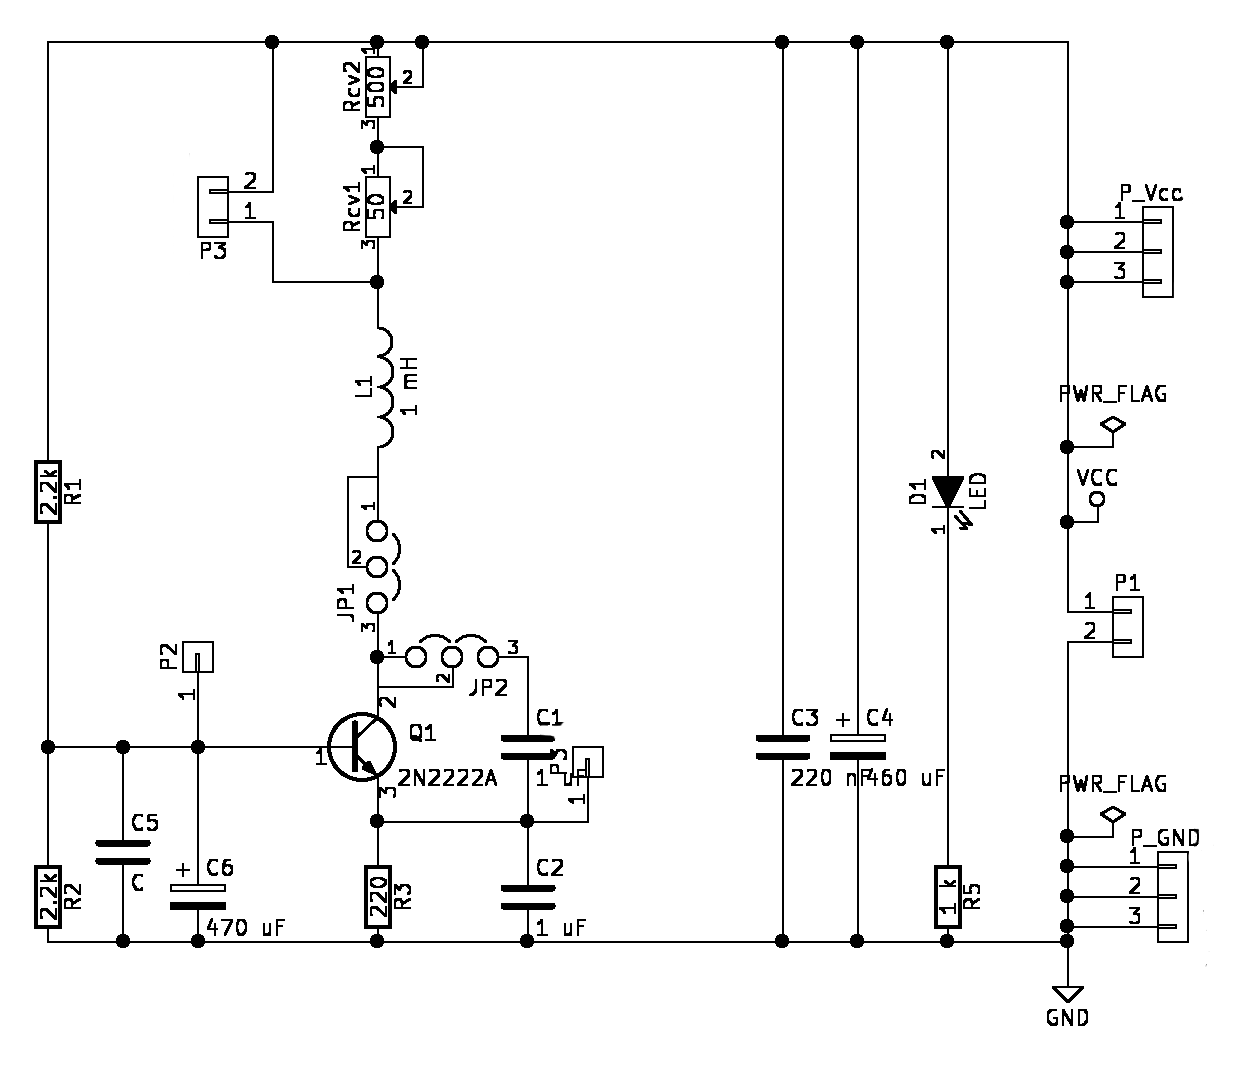
\includegraphics[width=0.8\textwidth]{p/colp_schem_real.png} }
\caption{Электрическая схема реального генератора Колпитца, используемого в данной работе}
\label{atu:f:colp_schem_real}
\end{figure}

Для стабилизации потенциалов $V_{cc}$ и $V_b$
в широком диапазоне частот использовались пары конденсаторов, соответственно
$\mathrm{C}_3$, $\mathrm{C}_4$ и
$\mathrm{C}_5$, $\mathrm{C}_6$. Конденсатор большей ёмкости
был электролитический, меньшей --- с керамическим диэлектриком.
Непосредственно в модели такой изменение схемы отражения не находит.
Напротив, эти изменения позволяют с меньшими допущениями считать
в модели вышеупомянутые потенциалы постоянными.

Резистор из исходной схемы $\mathrm{R}_c$,
в реальной схеме представлен двумя переменными резисторами
$\mathrm{R}_{cv1}$ и
$\mathrm{R}_{cv2}$. Это позволяет получить как широкий диапазон значений $\mathrm{R}_c$,
так и возможность тонкой настройки.
Следует отметить, что в полное сопротивление $\mathrm{R}_c$
входит и активное сопротивление катушки индуктивности $\mathrm{L}_{1}$.

Разъёмы $\mathrm{P}_1$, $\mathrm{P}_\mathrm{gnd}$ и $\mathrm{P}_\mathrm{Vcc}$
предназначены как для обеспечения электрическим питанием как самого генератора,
так и других приборов, которые участвуют в измерении.
Разъём $\mathrm{P}_4$ предназначен для получения сигнала $V_e(t)$.
Разъём $\mathrm{P}_2$ позволяет контролировать стабильность
потенциала $V_b$, однако, в процессе измерения этот сигнал не записывался.
Разъём с набором перемычек $\mathrm{JP}_2$, в первую очередь,
используется для получения сигнала $V_c$. Помимо этого,
он позволяет отключить от схемы конденсатор $\mathrm{C}_1$,
тем самым прекратить генерацию и исследовать поведение схемы в стационарном состоянии
для уточнения параметров.

Разъём с набором перемычек $\mathrm{JP}_1$ также выполняет несколько функций.
Убрав с него перемычку, можно измерить полное сопротивление $\mathrm{R}_{c}$,
что даёт возможность сравнить результат идентификации с реальным значением.
Также важным свойством является возможность с помощью этого разъёма
заменить пару $\mathrm{R}_{c}$, $\mathrm{L}_{1}$
на другую, что расширяет возможности эксперимента.

Разъём  $\mathrm{P}_{3}$, с одной стороны, позволяет
ввести параллельное сопротивление к
$\mathrm{R}_{cv1}$ и
$\mathrm{R}_{cv2}$, что необходимо для исследования динамических
свойств системы идентификации. С другой стороны,
измерение падения напряжения на измененном сопротивлении $\mathrm{R}_{cv1} +\mathrm{R}_{cv2}$
позволяет оценить величину $I_c(t)$, эквивалент безразмерной величины $y(t)$.
В этом случае нельзя говорить об идентификации, но данный сигнал может быть полезен
при построении аттрактора по наблюдаемым данным.


Принципиальная схема и печатная плана были спроектированы в
программном комплексе ``kicad''. % TODO: ref
Печатная плата изготовлена с использованием негативного фоторезиста.
Внешний вид собранной схемы на печатной плате представлен на~(рис.~\ref{atu:f:relax3d_board}).

\begin{figure}[htb!]
\centerline{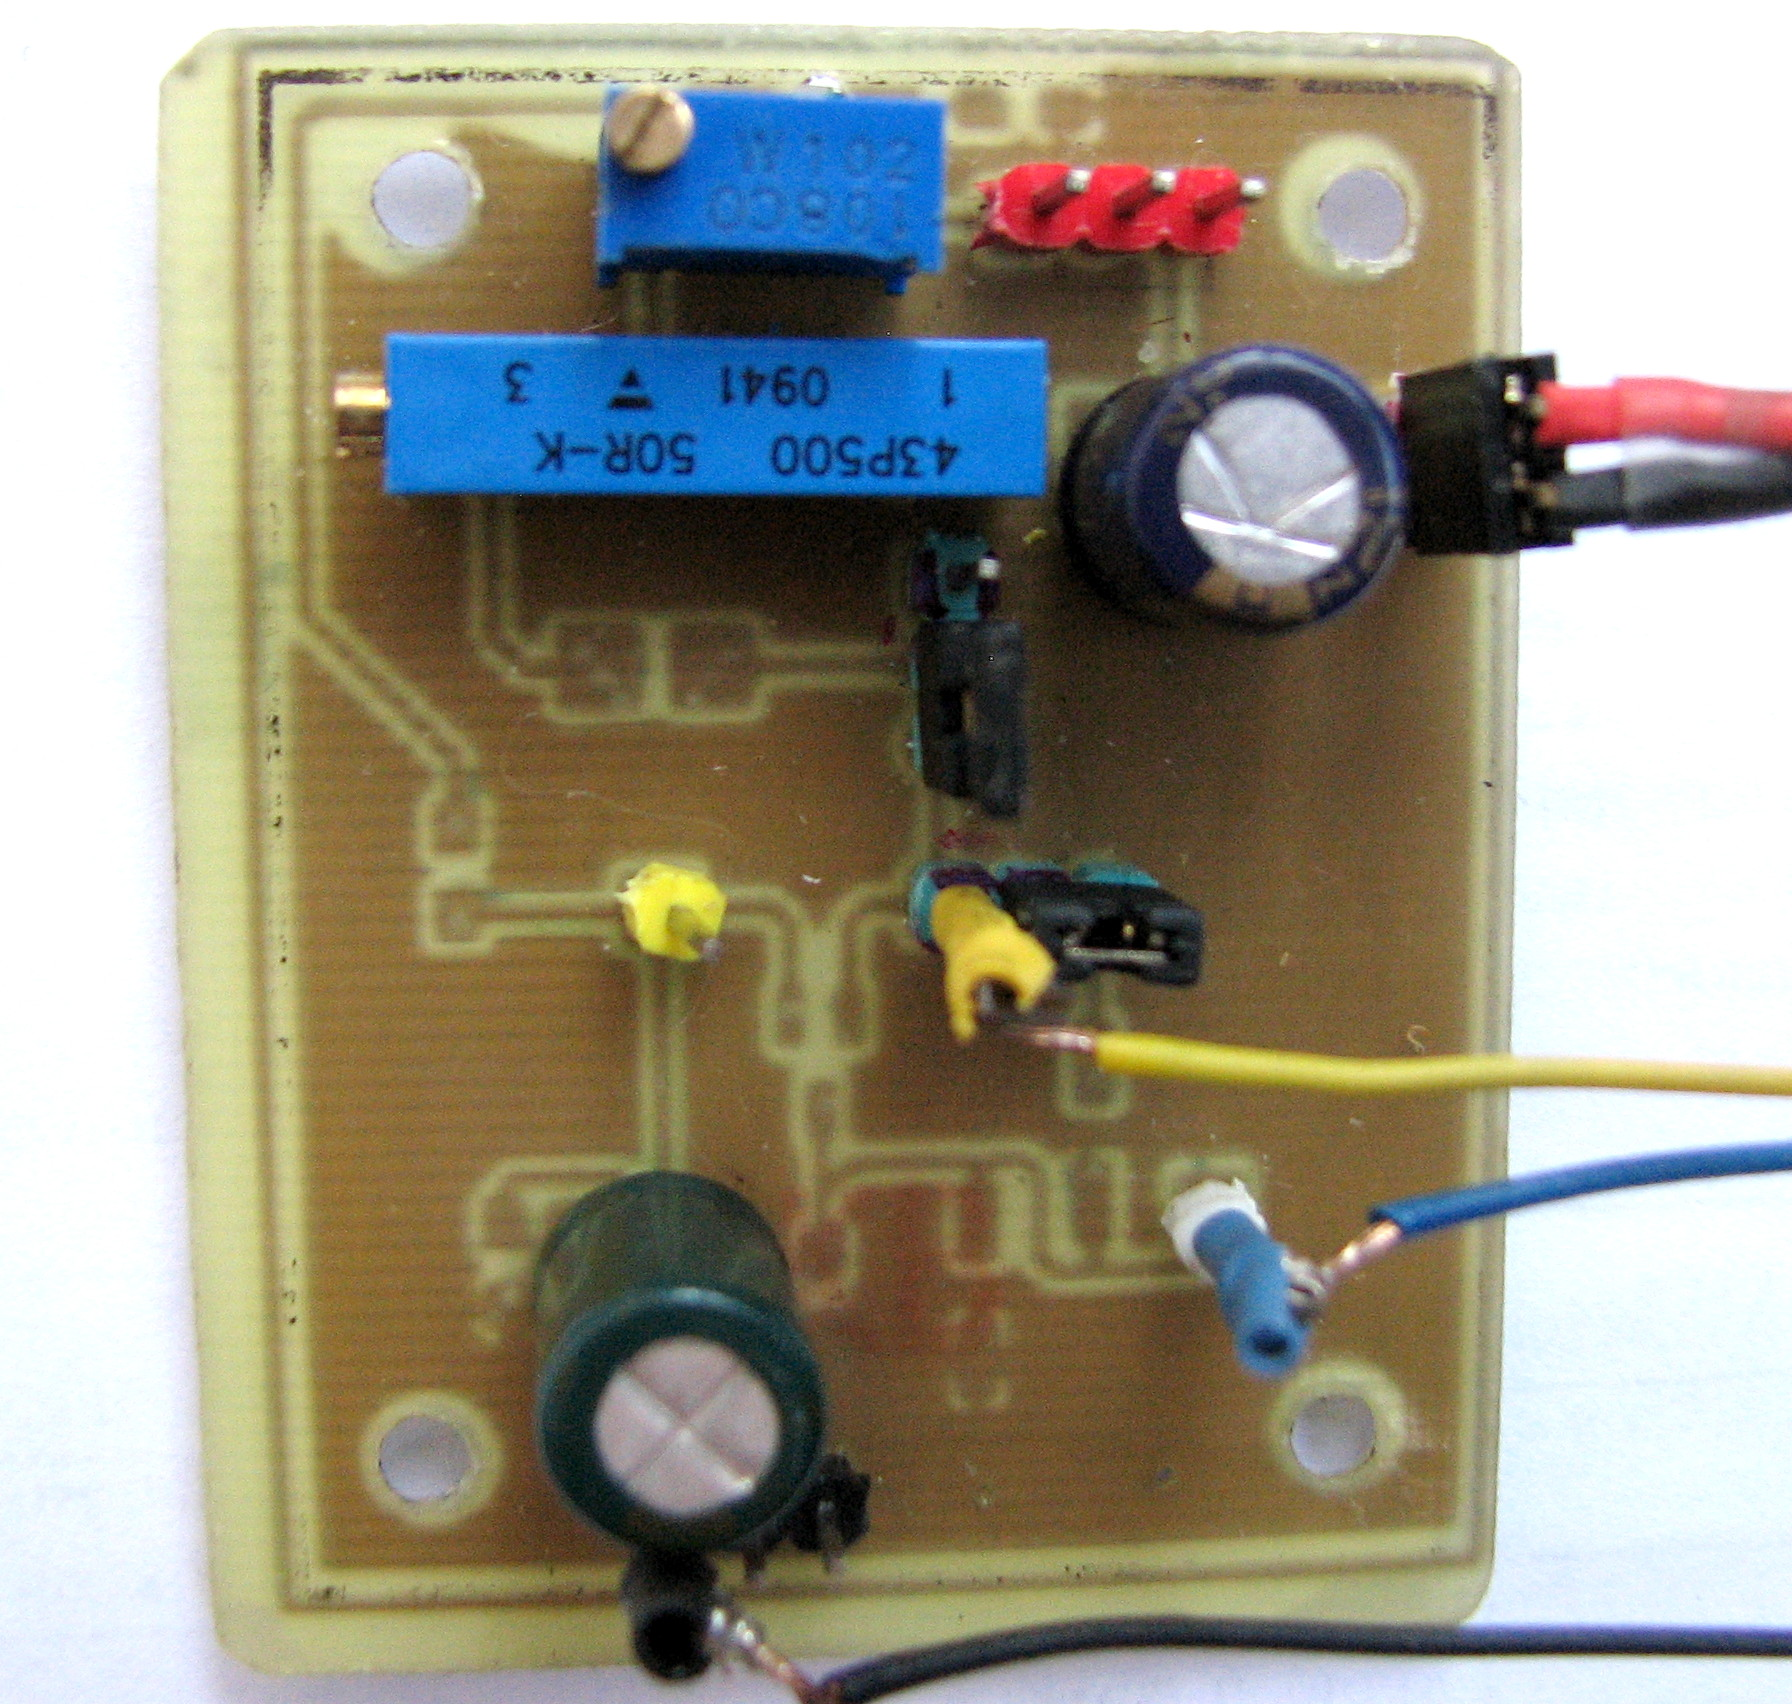
\includegraphics[width=0.5\textwidth]{p/colp_board.jpg} }
\caption{Печатная плата генератора Колпитца}
\label{atu:f:colp_board}
\end{figure}

Параметры всех элементов, существенных для функционирования системы,
были измерены до их установки на печатную плату.

% }}}1

\section{Моделирование динамики классической модели системы Колпитца и сравнение с реальным генератором}  % {{{1

Для оценки адекватности рассматриваемой модели были проведены серии как
вычислительных, так и натурных физических экспериментов.
Моделирование проводилось в программе ``qontrol''.
Для получения данных с реального генератора был использован цифровой осциллограф
Rigol DS1052E. % TODO: ref
С его помощью были получены как визуальные представления
аттракторов, так и оцифрованные значения сигналов $V_e(t)$ и $V_c(t)$.
На предварительном этапе были определены области простых и сложно-периодических колебаний,
а также область чередования хаотических и сложно-периодических колебаний.

При физическом моделировании, проведённом в рамках данной работы использовались следующие
элементы с соответствующими параметрами:
%
\[
  V_{cc} = \SI{12.06}{\volt},          \;
  R_1 = R_2 = \SI{2.2}{\kilo\ohm},     \;
  R_e = \SI{430}{\ohm},
\]
%
\[
  C_1 = C_2 = \SI{1.03}{\micro\farad}, \;
  L = \SI{6.22}{\milli\henry},         \;
  T = \SI{305}{\kelvin},
\]
%
\[
  \text{Q: 2N2222A}, \quad
  h_{fe}=285, \;
  V_f = \SI{0.677}{\volt}, \;
  I_s = \SI{9.61e-14}{\ampere}, \;
  \alpha \approx 1.
\]

Тогда безразмерные коэффициенты:
\[
 a = 77,     \quad
 c = 18.08,  \quad
 d = 0.19,   \quad
 e = 9.07.
\]
%
\[
F(z) =
\begin{cases}{l}
  e-1-z, & z \le e-1  \\
  0,     & z  >  e-1
\end{cases}.
\]

Диапазон изменения идентифицируемого параметра
$b \in [ 0.02; 4.2 ]$
определяется, с одной стороны, собственным сопротивлением катушки индуктивности,
с другой -- срывом генерации.

На рис.~\ref{atu:f:colp_real_xzz}--\ref{atu:f:colp_model_f} представлены как результаты реального эксперимента,
так и данные, полученные в результате численного моделирования динамики системы (\ref{atu:eq:colp}).
Представлены проекции аттракторов на плоскость $(x+z,z)$ (естественный вид для осциллографа),
трёхмерный вид аттракторов, и спектры.
На каждом рисунке представлено три режима: обычный, момент первого удвоения периода и хаотический режим.


\begin{figure}[htb!]
 \centerline{
   \includegraphics[width=0.32\textwidth]{p/mod/colp_m1_vv.png}
   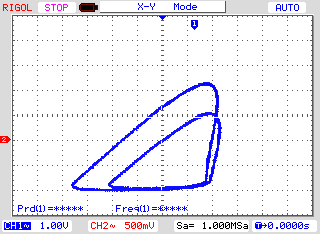
\includegraphics[width=0.32\textwidth]{p/mod/colp_m2_vv.png}
   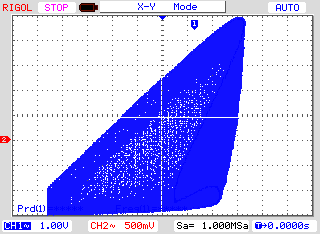
\includegraphics[width=0.32\textwidth]{p/mod/colp_m3_vv_ac.png}
 }
  \caption{Проекции аттракторов реальной системы Колпитца на плоскость $(x+z,z)$
  для трёх режимов}
  \label{atu:f:colp_real_xzz}
\end{figure}

Следует отметить, что при проведении измерений осциллограф
смог определить частоту колебаний только для режима простых колебаний.


\begin{figure}[htb!]
 \centerline{
   \includegraphics[width=0.32\textwidth]{p/mod/colp_0-p_z_xpz_b=1x70.png}
   \includegraphics[width=0.32\textwidth]{p/mod/colp_0-p_z_xpz_b=1x37.png}
   \includegraphics[width=0.32\textwidth]{p/mod/colp_0-p_z_xpz_b=0x99.png}
 }
  \caption{Проекции аттракторов модели (\ref{atu:eq:colp}) системы Колпитца на плоскость $(x+z,z)$
  для трёх режимов}
  \label{atu:f:colp_model_xzz}
\end{figure}




\begin{figure}[htb!]
 \centerline{
   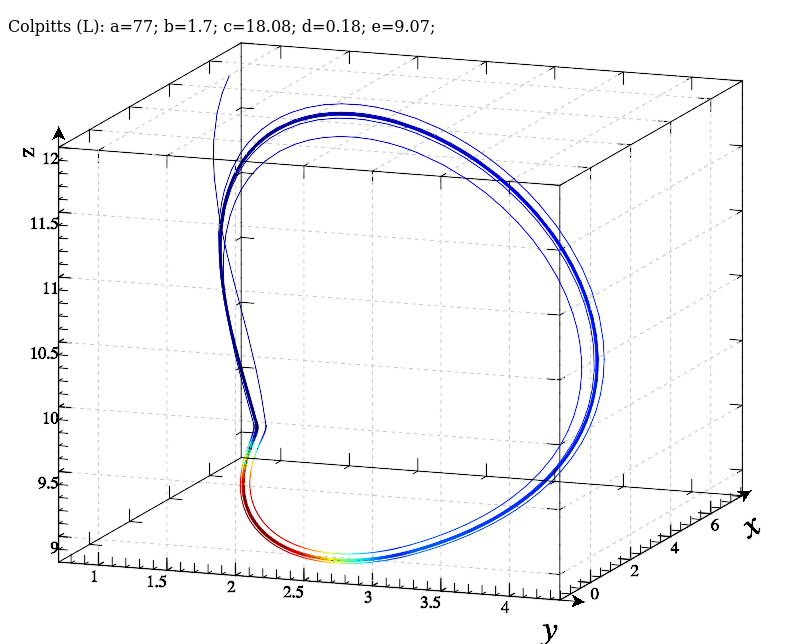
\includegraphics[width=0.32\textwidth]{p/mod/colp_0-p_xyz_b=1x70.png}
   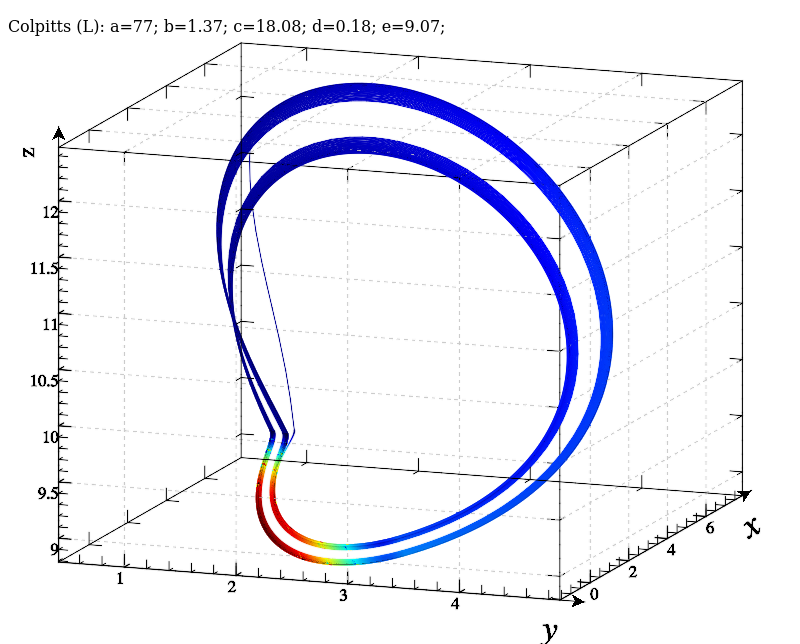
\includegraphics[width=0.32\textwidth]{p/mod/colp_0-p_xyz_b=1x37.png}
   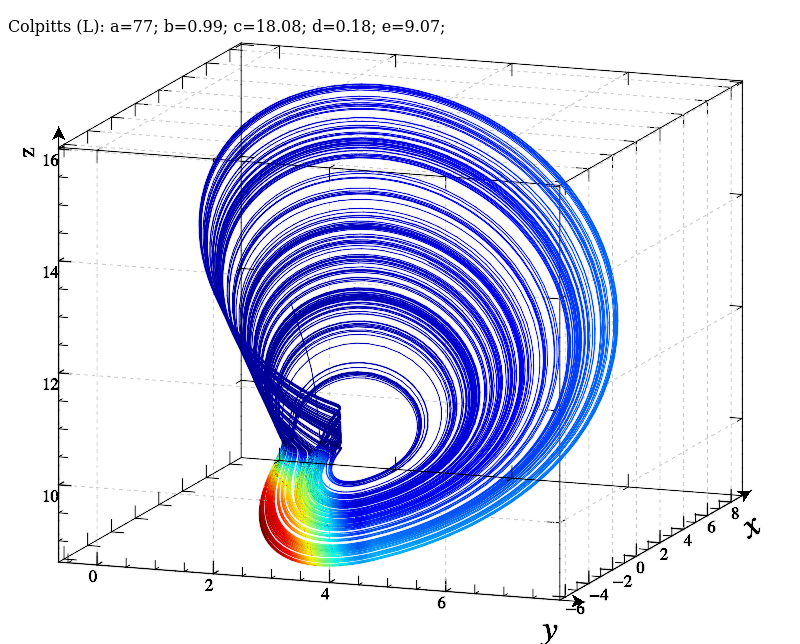
\includegraphics[width=0.32\textwidth]{p/mod/colp_0-p_xyz_b=0x99.png}
 }
  \caption{Аттракторы модели (\ref{atu:eq:colp}) системы Колпитца для трёх режимов}
  \label{atu:f:colp_model_xyz}
\end{figure}

\begin{figure}[htb!]
 \centerline{
   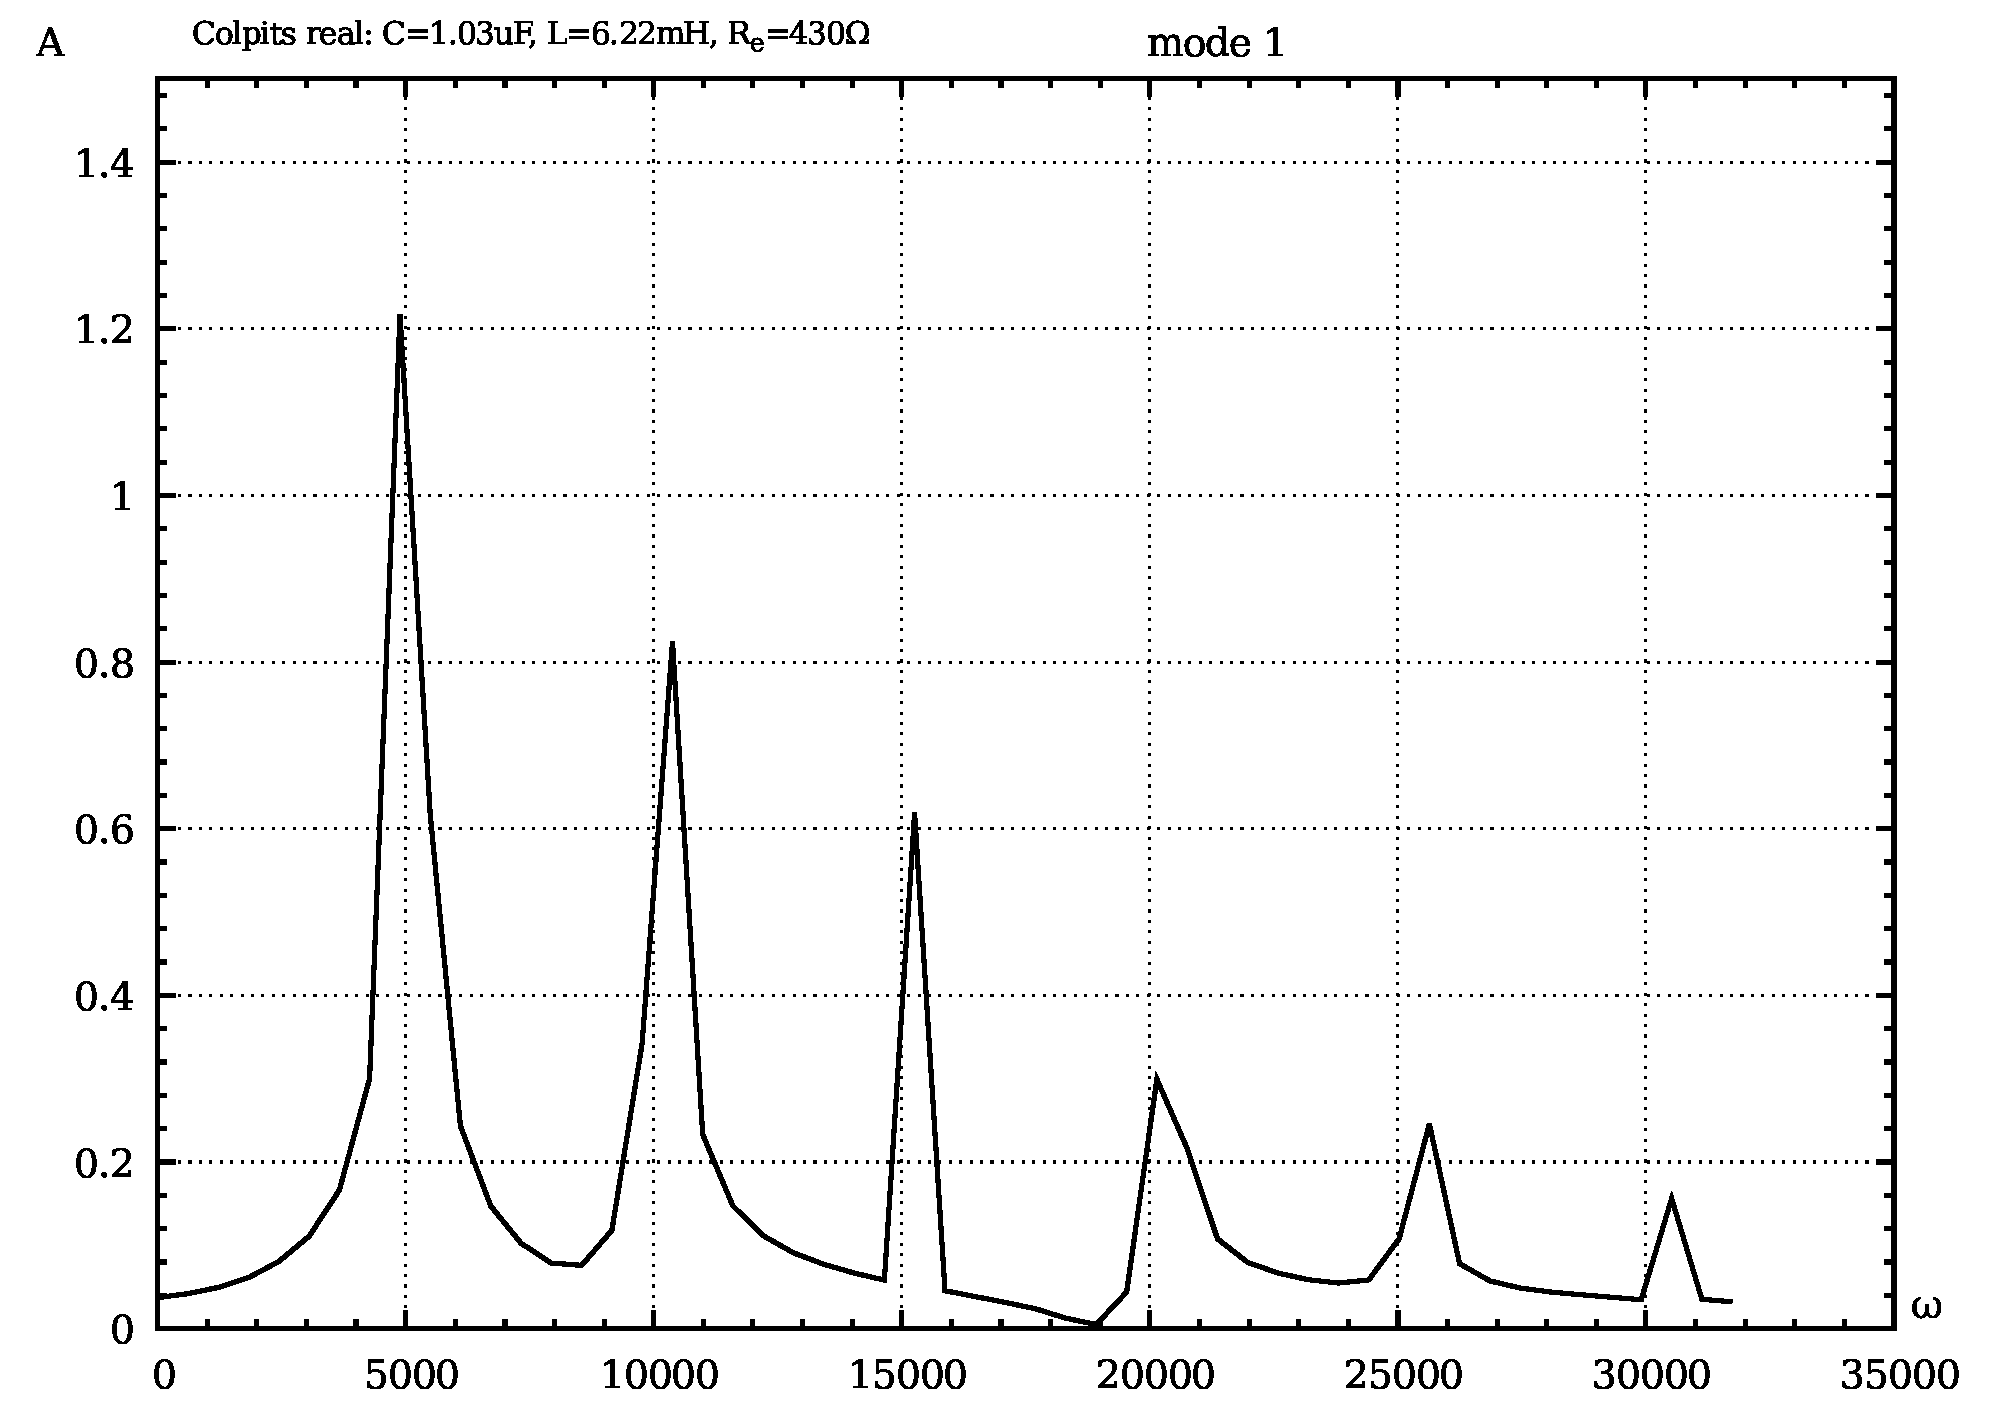
\includegraphics[width=0.32\textwidth]{p/mod/colp_m1_f.png}
   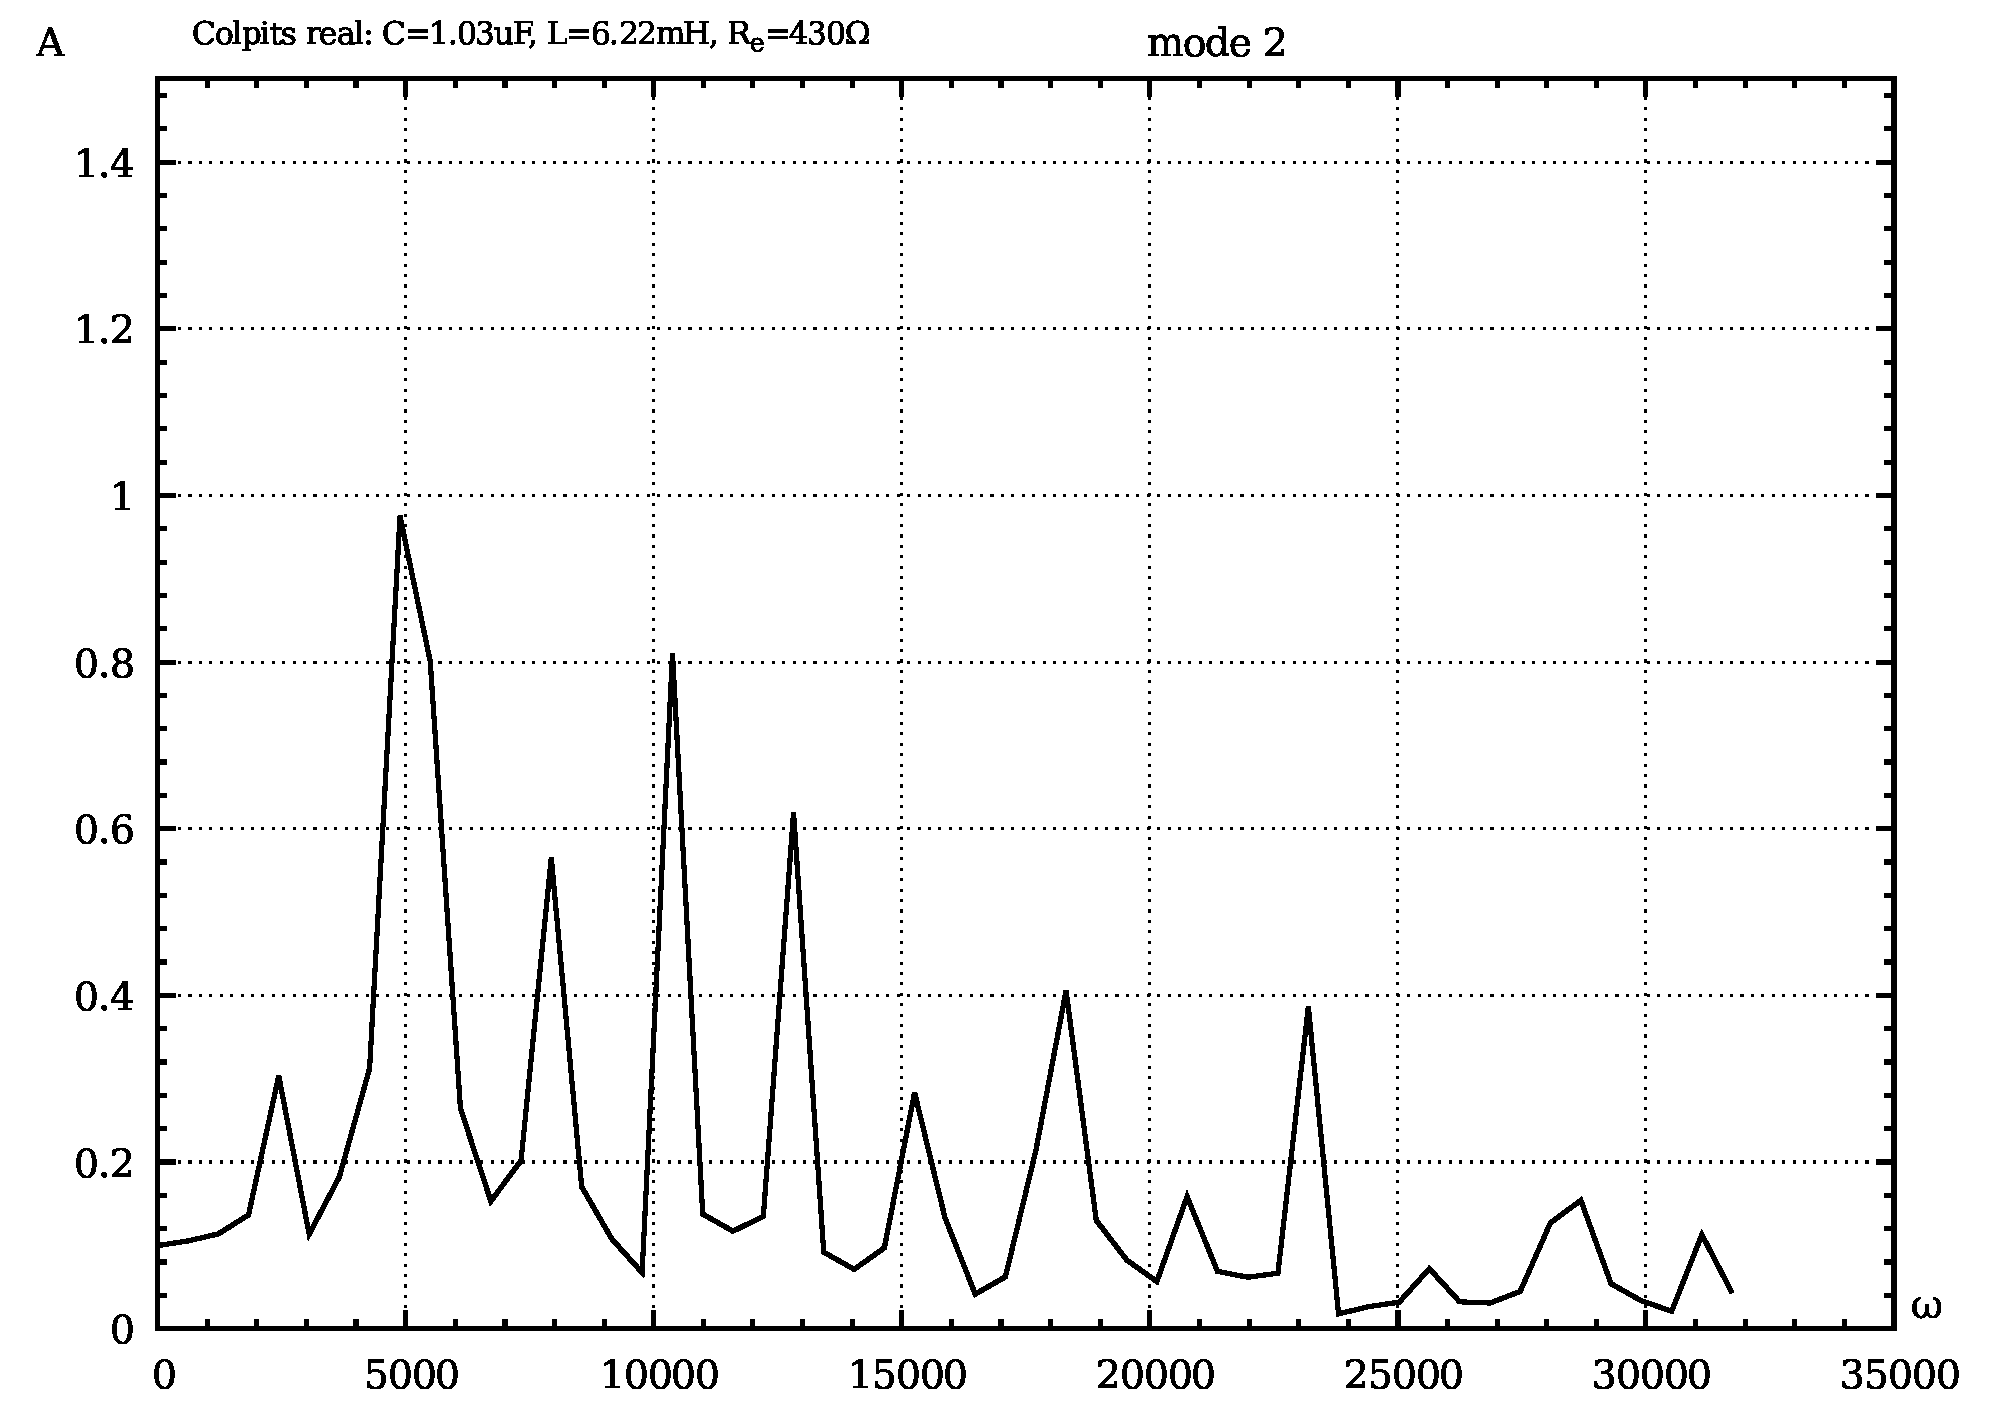
\includegraphics[width=0.32\textwidth]{p/mod/colp_m2_f.png}
   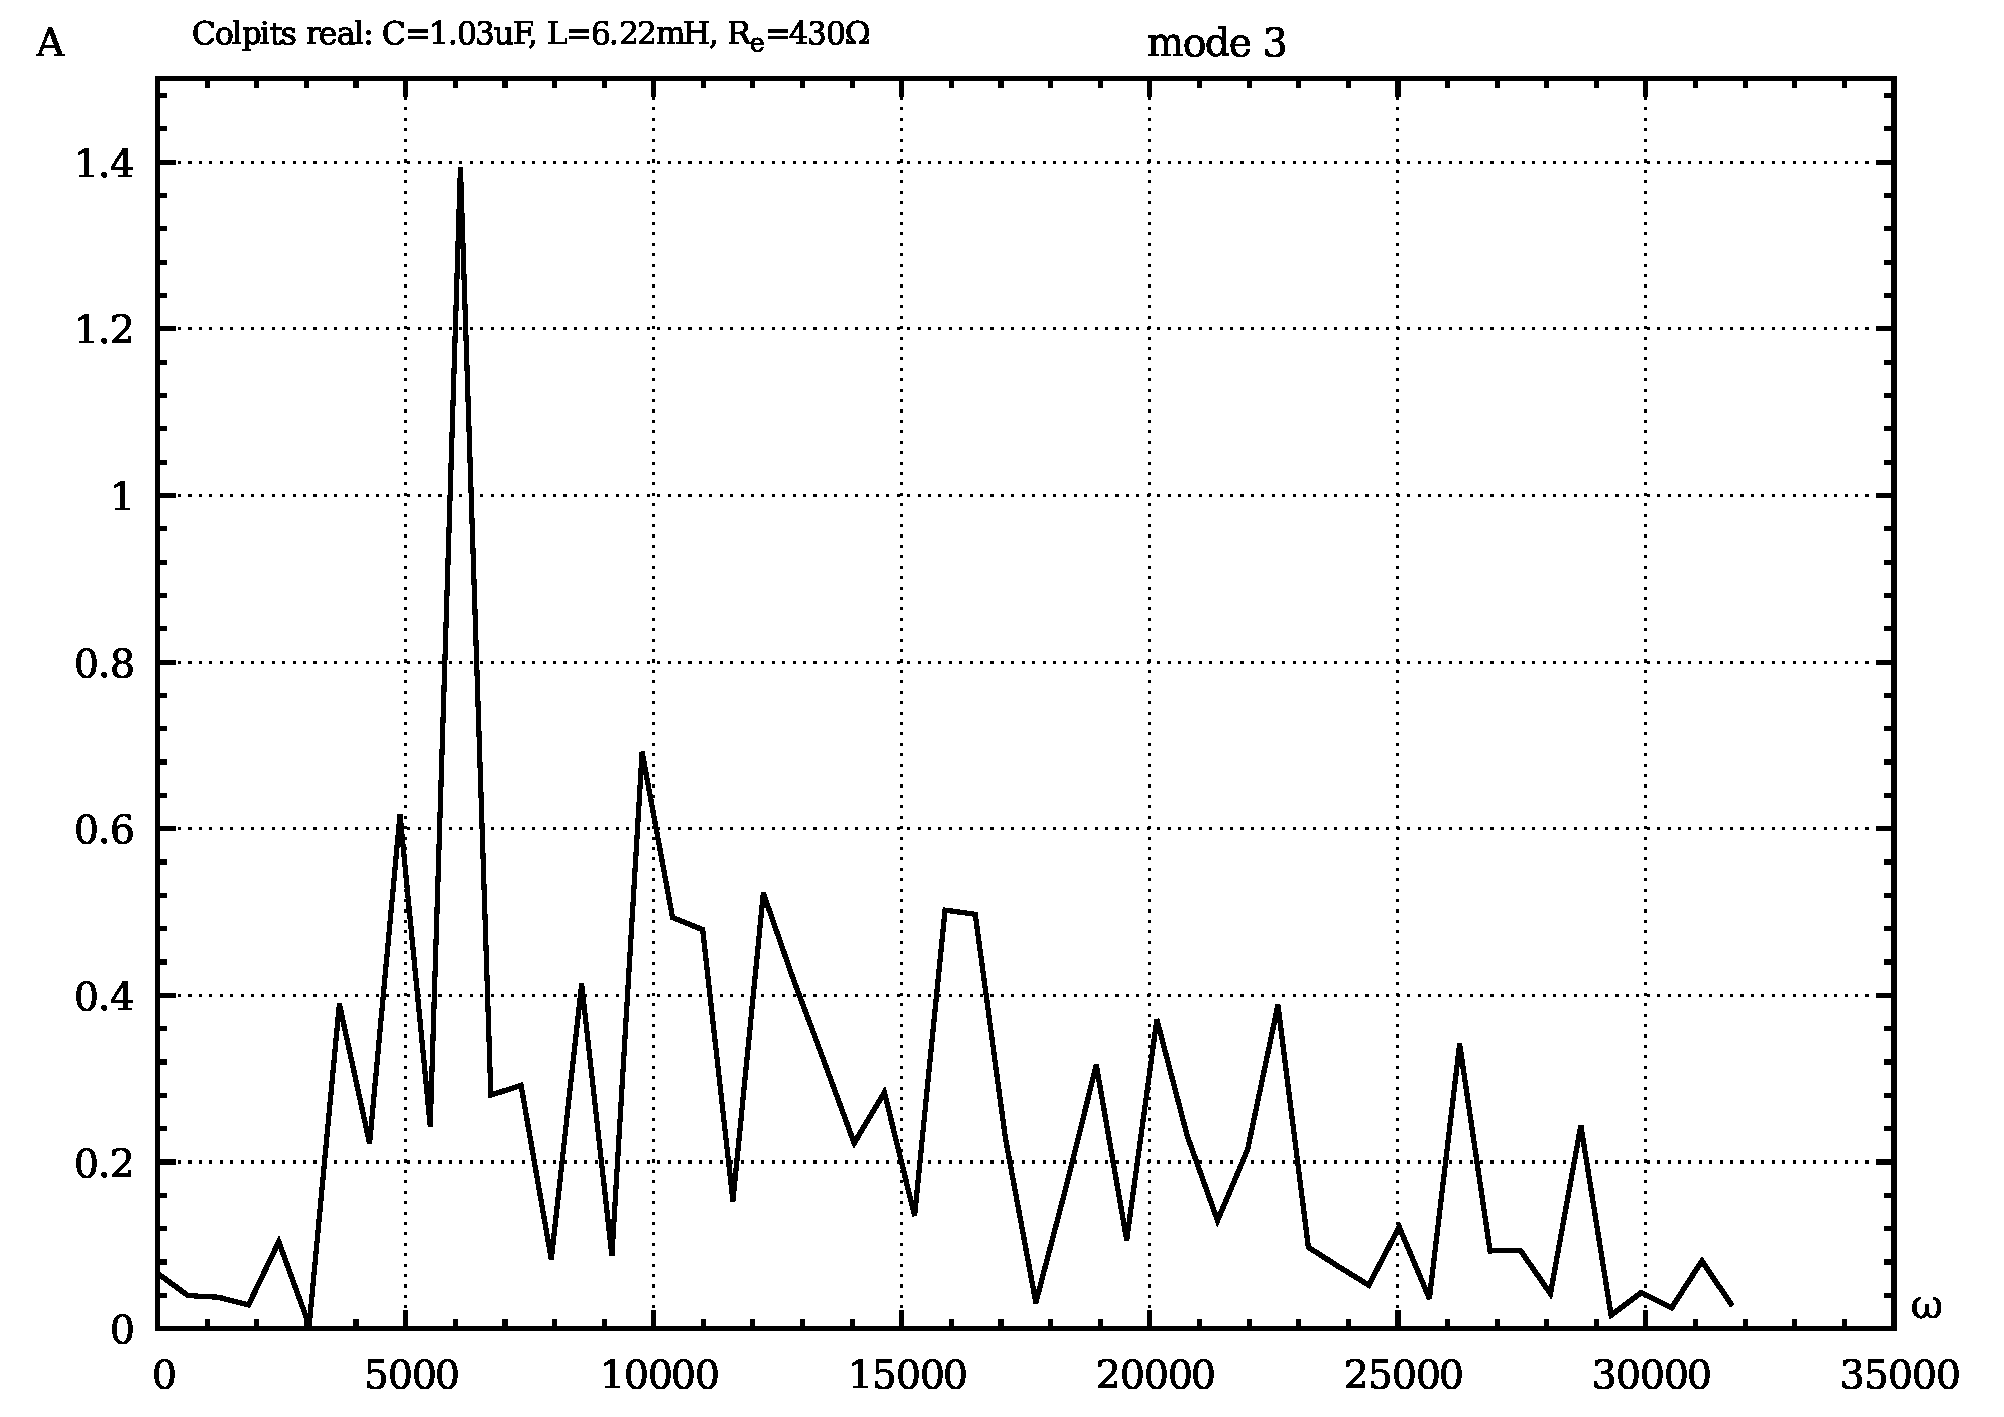
\includegraphics[width=0.32\textwidth]{p/mod/colp_m3_f.png}
 }
  \caption{Спектры реальной системы Колпитца  для трёх режимов}
  \label{atu:f:colp_real_f}
\end{figure}

\begin{figure}[htb!]
 \centerline{
   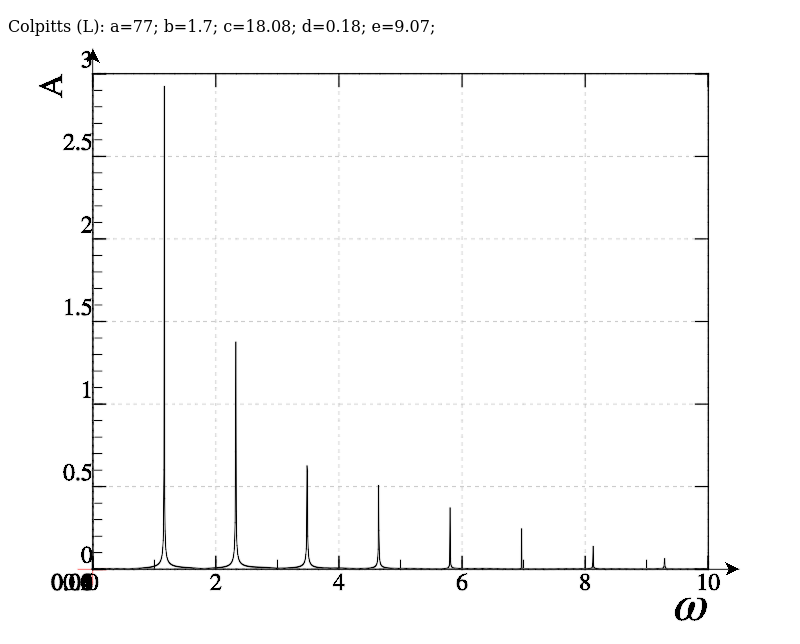
\includegraphics[width=0.32\textwidth]{p/mod/colp_f-p_f_b=1x70.png}
   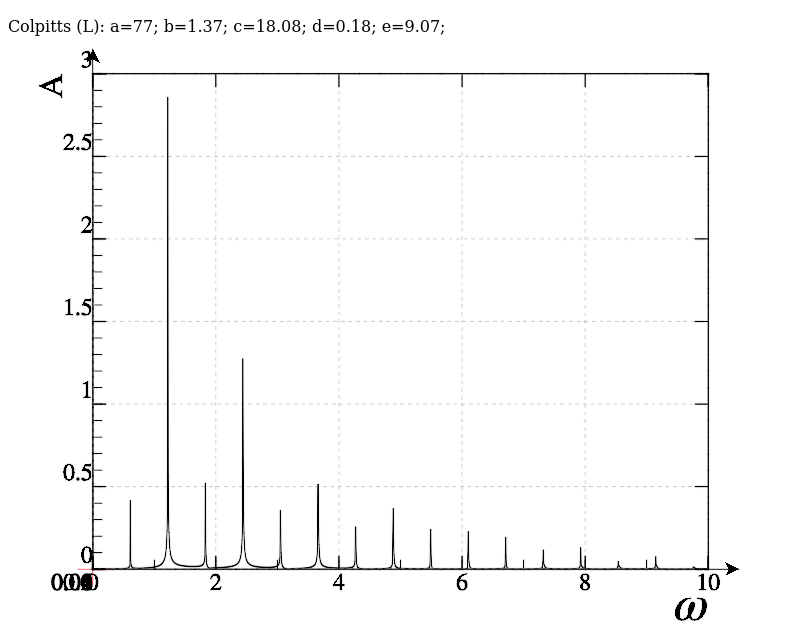
\includegraphics[width=0.32\textwidth]{p/mod/colp_f-p_f_b=1x37.png}
   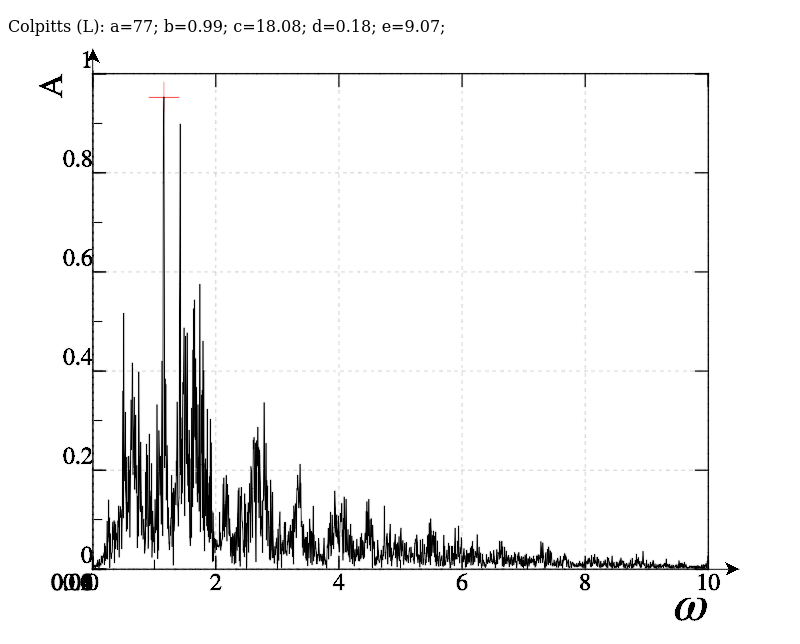
\includegraphics[width=0.32\textwidth]{p/mod/colp_f-p_f_b=0x99.png}
 }
  \caption{Спектры модели (\ref{atu:eq:colp}) системы Колпитца для трёх режимов}
  \label{atu:f:colp_model_f}
\end{figure}

Сравнение результатов физического и численного моделирования позволяет сделать вывод
о качественном подобии поведения реальной системы и модели.
Тем не менее, величины параметра $b$, при которых получены
рассматриваемые режимы, совпадают весьма приближённо.
Для реальной системы значения параметра: $b = 1.06, \; 0.94, \; 0.90 $, в то время как
для модели: $b = 1.70, \; 1.34, \; 0.99 $.
Расхождение значений, скорее всего, связано с грубостью модельного представления (\ref{atu:eq:bjt_libear_model}) транзистора.
Вопрос применимости различных моделей биполярного транзистора в рамках рассматриваемой системы
требует дальнейшего исследования.
С другой стороны, ограниченный набор данных, получаемых с осциллографа  (8192 отсчёта) не позволяют
получить достаточно подробный спектр реальной системы.
Разрешение в спектральной области составляет $ \approx \SI{190}{\hertz}$.

% }}}1

\section{Критерии идентификации для классической модели системы Колпитца}  % {{{1

Несмотря на только качественное подобие модели (\ref{atu:eq:colp})
и реальной системы, построим систему идентификации
и использованием только моделей данного вида.
Это позволит определить возможность идентификации
для широко используемого в литературе приближения.

Для определения критерия идентификации рассмотрим зависимости
$q(b) $, полученные путём моделирования
для системы Колпитца (рис.~\ref{atu:f:colp_q}).
При этом следует учесть, что наиболее просто измеряемыми величинами являются $x$ и $z$,
соответствующие напряжениям $V_1$ и $V_2$.
Первый набор зависимостей даёт два основных кандидата -- $q_{x^2}$ и $q_{z^2}$.
При этом первый из них показывает более равномерную зависимость.
В то же время, большинство из рассмотренных зависимостей имеют явно
выраженный гиперболический характер, особенно при малых значениях $b$.
Следовательно, в список кандидатов следует добавить $q_{x^{-2}} $ и $q_{z^{-2}}$.

\begin{figure}[htb!]
\centerline{
  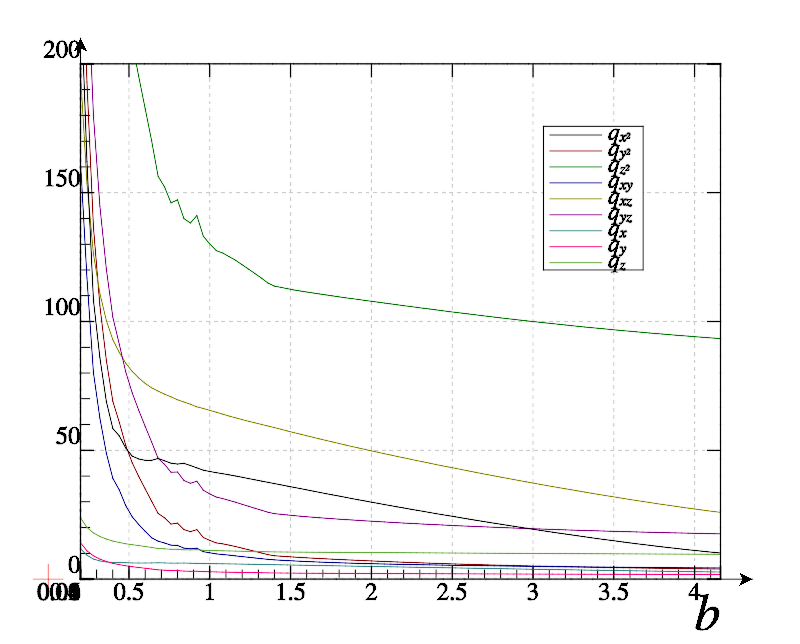
\includegraphics[width=0.49\textwidth]{p/mod/colp_p-p_b_e.png}
  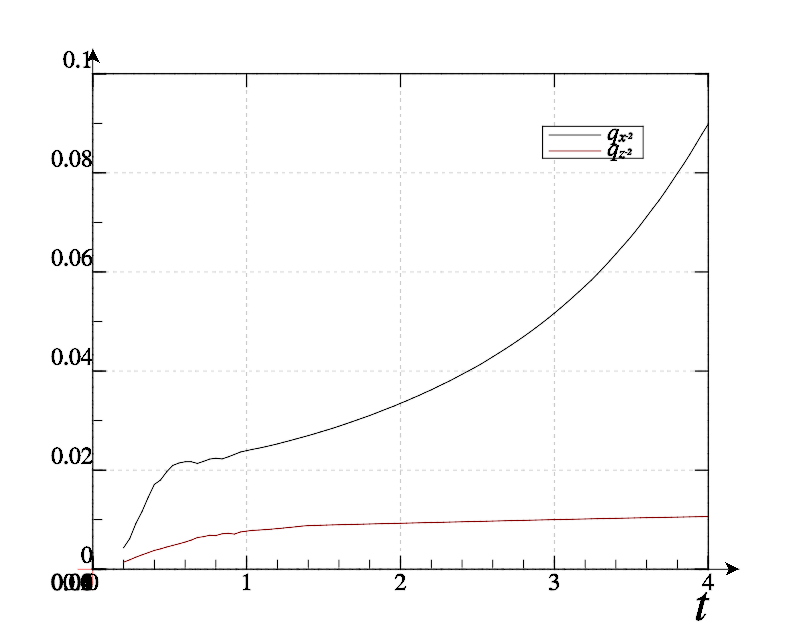
\includegraphics[width=0.49\textwidth]{p/mod/colp_p-p_b_1ex2.png}
}
  \caption{Зависимости $q(b) $ для системы Колпитца (\ref{atu:eq:colp})}
\label{atu:f:colp_q}
\end{figure}

Из графиков очевидно, что
обратные зависимости не дают заметного выигрыша, поэтому выберем
величину $ q_{x^2}(b) $ в качестве критерия.

% }}}1

\section{Моделирование процессов идентификации для классической модели генератора Колпитца} % {{{1

% TODO: new name
В качестве системы идентификации использовалась система с пятью поисковыми агентами и
двумя неподвижными моделями.
Согласно введённой классификации, метод обозначается как  Fq3rlovngcF.$q_{x^2}$:5.
Аналогично предыдущим системам,
для исследования динамических свойств системы идентификации
изменения параметра $b_o$ как:
%
\begin{equation}
 b_o(t) = p_0 + U_p \sign \sin( \omega_p t ),
  \label{atu:eq:colp_b_sign}
\end{equation}
%
\begin{equation}
 b_o(t) = p_0 + U_p \sin( \omega_p t ).
  \label{atu:eq:colp_b_sin}
\end{equation}

Динамика процессов идентификации для системы Колпитца представлена на рис.~\ref{atu:f:colp_id}.

\begin{figure}[htb!]
\centerline{
  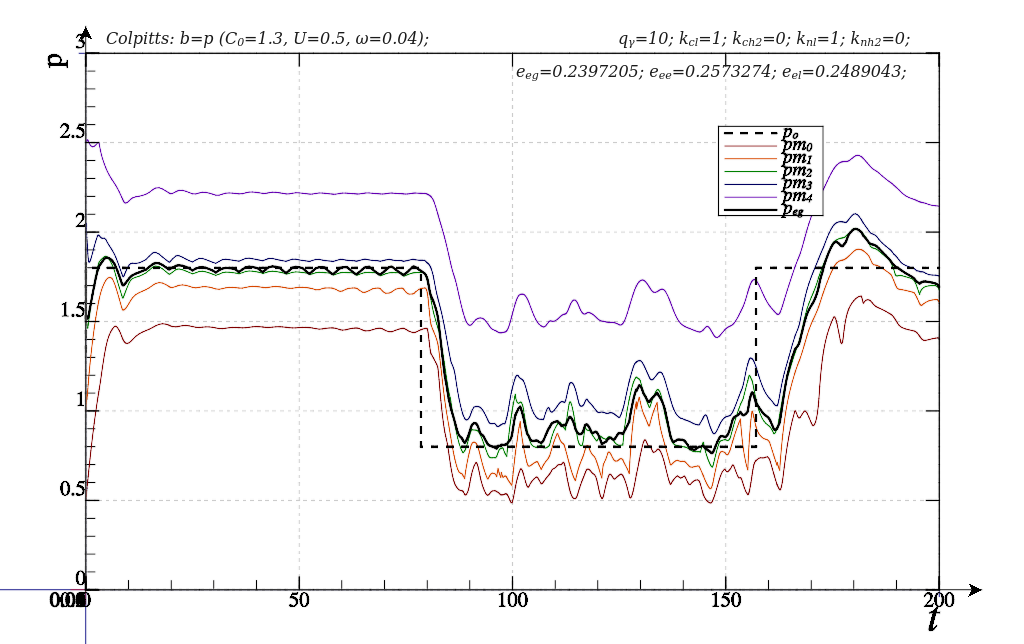
\includegraphics[width=0.49\textwidth]{p/mod/colp_m5p-pl_n_sign.png}
  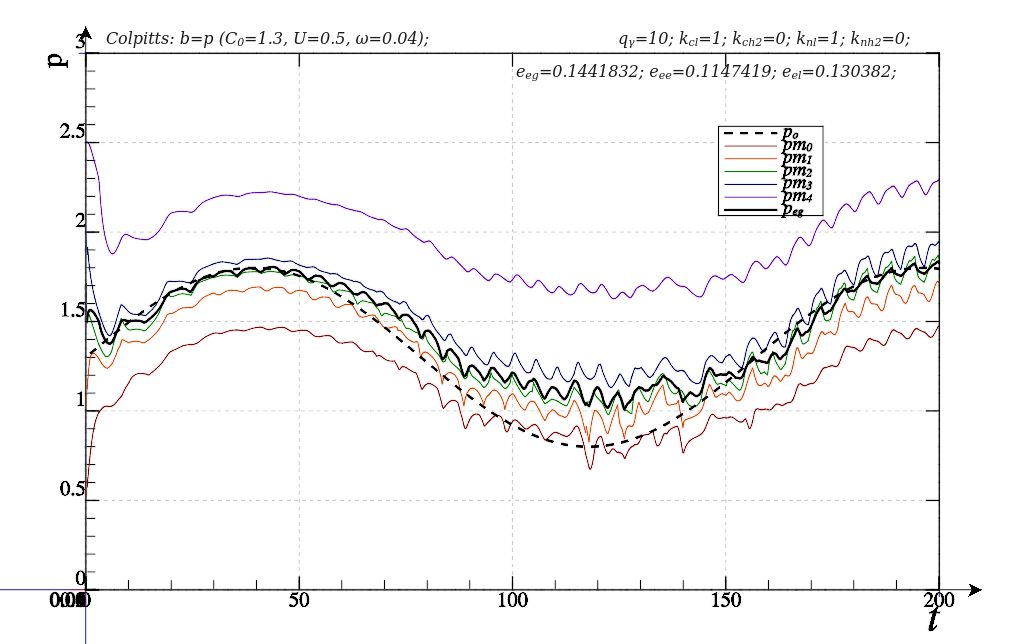
\includegraphics[width=0.49\textwidth]{p/mod/colp_m5p-pl_n_sin.png}
}
\caption{Процесс идентификации параметра $b$ системы (\ref{atu:eq:colp})
  при условиях (\ref{atu:eq:colp_b_sign}) и (\ref{atu:eq:colp_b_sin})
}
\label{atu:f:colp_id}
\end{figure}

Анализ полученных графиков позволяет сделать вывод,
что система идентификации получилась вполне работоспособной.
Обращает на себя внимание рост ошибки идентификации при относительно малых
значения параметра $b$. Тем не менее, с учётом только качественного подобия
рассматриваемой модели этим явлением вполне можно пренебречь.

% }}}1

\section{Влияние параметров системы идентификации на ошибку идентификации для классической модели системы Колпитца}  % {{{1

Зависимости $\overline{e}(a_q)$ (рис.~\ref{atu:f:colp_e_a_q})
позволяют корректно определить время усреденения.
При этом следует отметить, что
полученные результаты хорошо согласуются со спектрами системы.

\begin{figure}[htb!]
\centerline{
  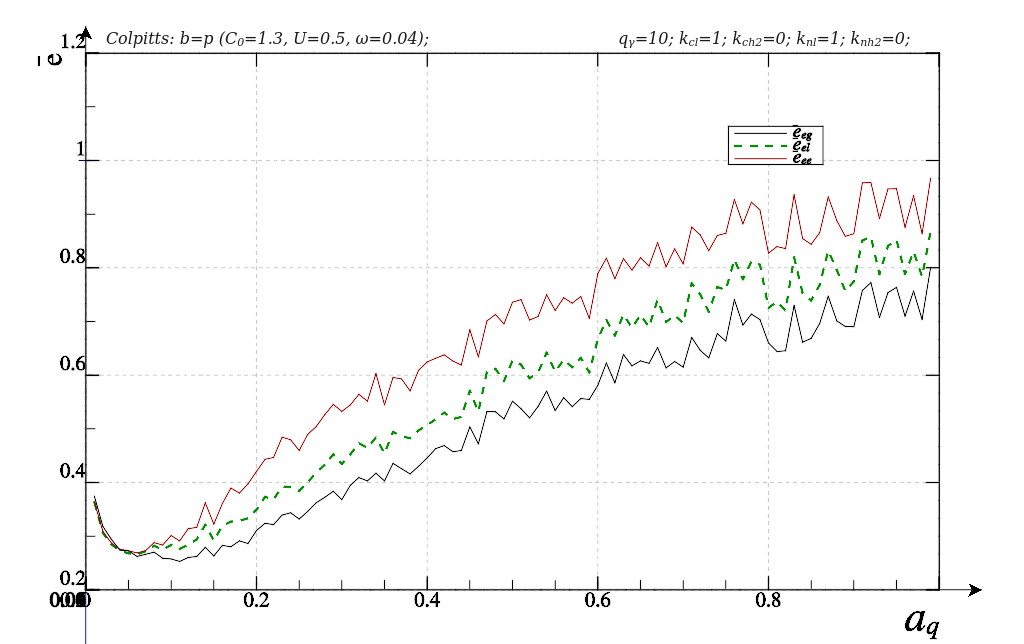
\includegraphics[width=0.49\textwidth]{p/mod/colp_m5p-p_a_q_e_sign.png}
  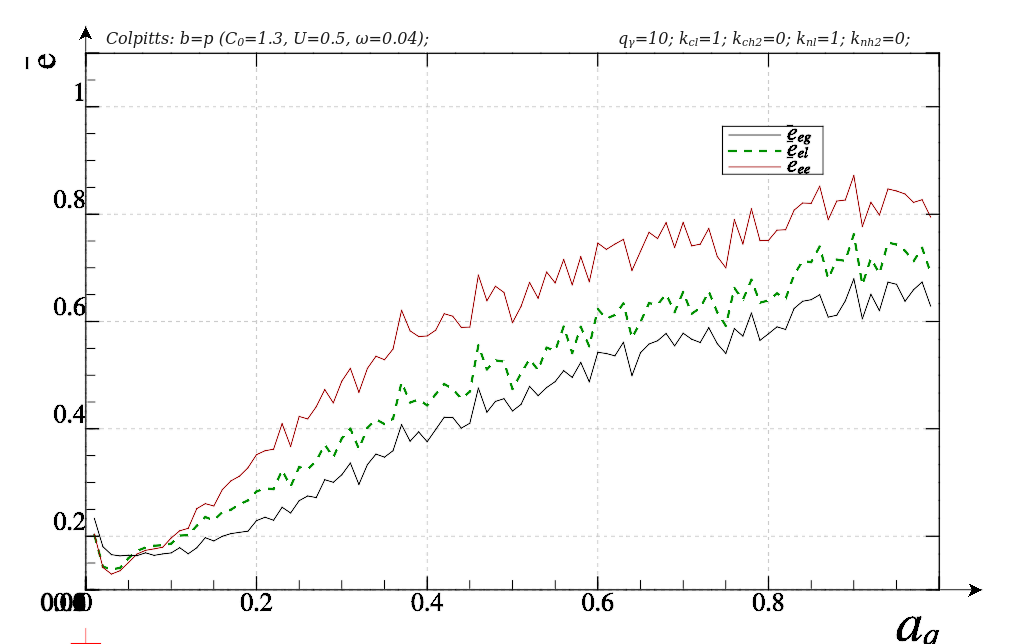
\includegraphics[width=0.49\textwidth]{p/mod/colp_m5p-p_a_q_e_sin.png}
}
  \caption{Зависимости  $\overline{e}(a_q)$ для системы (\ref{atu:eq:colp})
  при условиях (\ref{atu:eq:colp_b_sign}) и (\ref{atu:eq:colp_b_sin})
}
\label{atu:f:colp_e_a_q}
\end{figure}

Аналогично, зависимости среднеквадратических ошибок идентификации от величины $q_\gamma$ (рис.~\ref{atu:f:colp_e_qgamma})
даёт информацию о корректной настройке этого параметра системы идентификации.

\begin{figure}[htb!]
\centerline{
  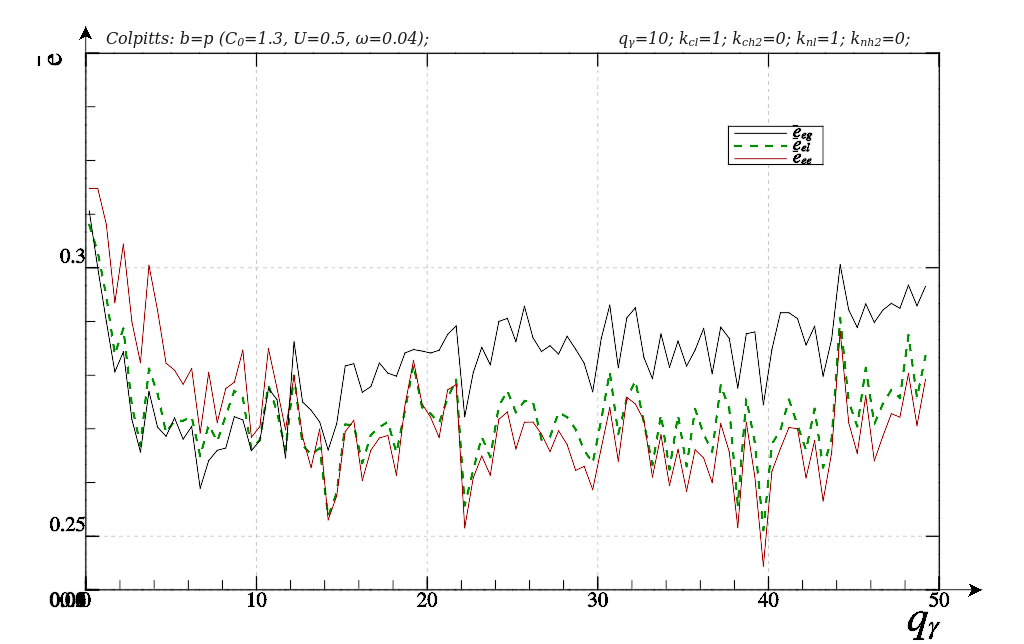
\includegraphics[width=0.49\textwidth]{p/mod/colp_m5p-p_qg_e_sign.png}
  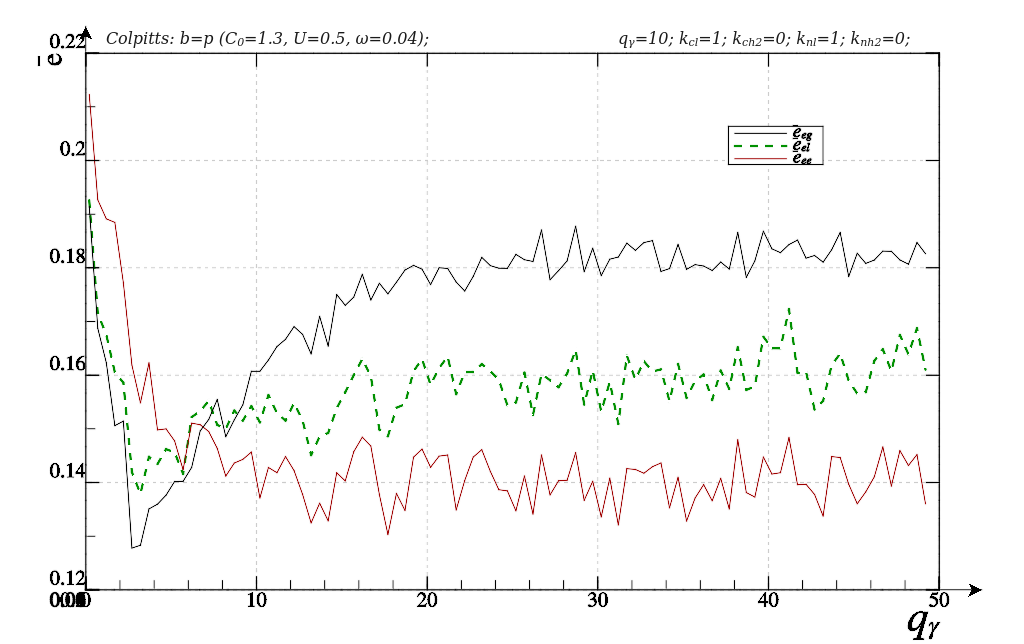
\includegraphics[width=0.49\textwidth]{p/mod/colp_m5p-p_qg_e_sin.png}
}
  \caption{Зависимости  $\overline{e}(q_\gamma)$ для системы (\ref{atu:eq:colp})
  при условиях (\ref{atu:eq:colp_b_sign}) и (\ref{atu:eq:colp_b_sin})
}
\label{atu:f:colp_e_qgamma}
\end{figure}

Более подробный анализ зависимостей для данной системы практически не имеет смысла,
ввиду ограниченности модели.




% }}}1



\section{Уточнённая модель генератора Колпитца}  % {{{1

Как уже было отмечено,
рассмотренная  модель
генератора Колпитца, несмотря на её широкое использование
при исследованиях, связанных с хаотической динамикой,
имеет существенные отличия от реального генератора.
Подавляющие большинство элементов достаточно хорошо описываются линейным
приближением. Однако, есть два элемента,
применение линейной модели для которых или же вообще невозможно (транзистор),
или же допустимо при определённых условиях (индуктивность).

Как уже было упомянуто, более точной моделью транзистора является представление
Эберса-Молла~\cite{horowitz}:
%
\begin{equation}
  I_c = I_s \left( \exp\frac{V_{be}}U_t{} - 1 \right),
  \label{atu:eq:ebers-moll}
\end{equation}
%
%\noindent
где
$I_s$ -- ток насыщения (паспортная или определяемая экспериментально величина),
$U_t=kT/q$,
$q = \SI{1.6e-19}{\coulomb}$ -- заряд электрона,
$k = \SI{1.38e-23}{\joule/\kelvin}$ -- постоянная Больцмана.
Необходимо учесть, что в режиме отсечки ($V_b < V_e$) ток коллектора пренебрежимо мал,
а в режиме насыщения определяется другими элементами схемы.


Существуют и более сложные модели, например,
программы для моделирования электронных схем часто используют так называемую SPICE модель.


% }}}1

\section{Исследование динамики физической реализации генератора Колпитца} % {{{1


Как уже отмечалось, использование в качестве регистратора данных
цифрового осциллографа класса Rigol DS1052E,
несмотря на  хорошее разрешение во временной области ($\SI{10}{\nano\second}$),
скорость и простоту получения вида аттрактора,
имеет ряд существенных недостатков.

В первую очередь, за исключением режима предельной частоты дискретизации,
нет возможности получить достаточно длинную выборку, что
сильно ограничивает возможности спектрального анализа.
При анализе сигналов хаотических и близких к ним систем
особенно важным является спектральное разрешение,
определяемое количеством наблюдений при заданной частоте дискретизации.
При недостаточном разрешении нет способа отличить участок сплошного спектра
от линейчатого.

Также, ограниченная разрядность входных АЦП (8 бит)
приводит к относительно высокому уровню шумов квантования.
Также, наличие только двух каналов измерения не позволяет
получить вид аттрактора для системы с тремя измерениями.

Для устранения этих недостатков был создан
измерительный комплекс на основе
микроконтроллера STM32F746.
Ядром системы служила отладочная плата Waveshare STM32F746.
Помимо собственно контроллера, на ней установлена оперативная память
SDRAM 8MB, что позволило сохранять в сумме до 4 миллионов отсчётов.
Использовалось до четырёх каналов 12-ти АЦП с разрешением 12 бит.
С учётом предела $2 \cdot 10^6$ отчётов в секунду
(с использованием DMA для пересылки полученных данных в память и таймера как сигнала для начала измерений),
максимальная достижимая частота дискретизации в этих условиях достигает $\SI{500}{\kilo\hertz}$,
что для исследуемой системы несколько избыточно,
но позволяет убедится в том, что не была потеряна часть спектра.

Для управления микроконтроллером была создана программа
на языке C++. Так как для данной задачи требуется
квази-одновременное, так и полностью одновременное выполнение
различных действий, то была использована миниатюрная операционная
система реального времени для микроконтроллеров FreeRTOS.
Управление программой осуществлялось в режиме терминала
с использование протокола UART. Реализованная
в программе система команд позволяет настраивать параметры измерения,
проводить само измерение, и сохранять результат.

В качестве основного способа сохранения результата
использовалась SDHC карта, подключенная по протоколу SDIO с одной линией данных.
Следует отметить, что при проведении измерения обязательным условием
является отключение SDIO подсистемы контроллера.
В противном случае уровень шумов измерения не позволяет
получить значимые результаты.
Альтернативным способом сохранение данных является
использование того же канала, который используется для передачи команд
и приёма ответа на них --- UART. Для сохранения результатов в файл
применяются средства используемой программы эмуляции терминала.
Однако, относительно низкая скорость такого способа передачи данных
требует длительного времени для сохранения результатов.

Важным условием получения данных является согласование уровней
сигналов в исследуемой системе с допустимыми входными уровнями АЦП.
Амплитудное значение сигналов в рассматриваемой системе достигало
$\SI{15}{\volt}$, в то время как входное напряжение АЦП не должно
превышать $\SI{3}{\volt}$.
Использование для согласования резистивного делителя
не оправданно. Малое полное сопротивление делителя
искажает динамику исследуемой системы, особенно в условиях
хаотических колебаний. Большие значения приводят
к росту шумов измерения и невозможности
использования защитных средств, например, пар диодов,
для защиты входных цепей контроллера.

Поэтому, для согласования использовалась микросхема TL074,
объединяющая в одном корпусе 4 операционных усилителя,
которые характеризуются высоким входным сопротивлением ($\approx \SI{1e12}{\ohm}$),
низким уровнем нелинейных искажений ($\approx 0.003\%$),
подходящим для данной задачи частотным диапазоном
и допустимыми входными напряжениями.
Каждый из усилителей включался в режиме повторителя~\cite{horowitz},
и на его выход был подключён резистивный делитель
с подобранными сопротивлениями и два защитных диода.

Перед каждой серией экспериментов проводилась калибровка
измерительного комплекса на набор заданных значений напряжений.
После измерений проводилась проверка на стабильность
параметров, и в случае отрицательного результата
данные отбрасывались.

В первой серии экспериментов значение параметра
$R_c$ было для каждого эксперимента фиксированным,
и настраивалось перед каждым экспериментом.
Использовался неравномерный ряд значений параметра в диапазоне $[ 25.3 ; 100]\SI{}{ohm} $.
В тех областях, где наблюдалось сложное поведение, расстояние между точками было меньшим.

Система регистрации данных работала с использованием четырёх
каналов измерения. Измерялись сигналы:
$V_e(t) = V_1(t)$,
$V_c(t) = V_1(t) + V_2(t)$,
$V_{ca}(t)$ --- потенциал на контакте 1 разъёма $\mathrm{P}_3$,
$V_cc(t)$.
Сигнал $V_2(t)$ определялся как $V_c(t) - V_e(t)$.
Ток через катушку индуктивности оценивался как
$I_L = \frac{V_{cc}(t) - V_{ca}(t)}{R_{cv1}+R_{cv2}}$.
Сигнал $V_{cc}(t)$ использовался для контроля калибровки
системы регистрации, а также для проверки отсутствия пульсаций напряжения питания.



При относительно высоких значения параметра $R_c$
наблюдается регулярная динамика и линейчатый спектр~(рис.~\ref{atu:f:colp_r_attr_f_50}).

\begin{figure}[htb!]
  \centerline{
    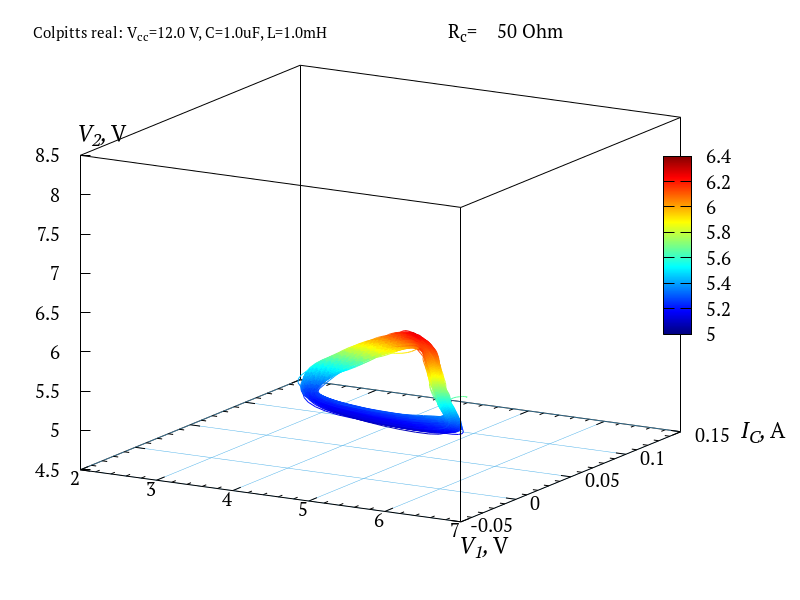
\includegraphics[width=0.48\textwidth]{p/r/v1iv2_050000.png}
    \hfill
    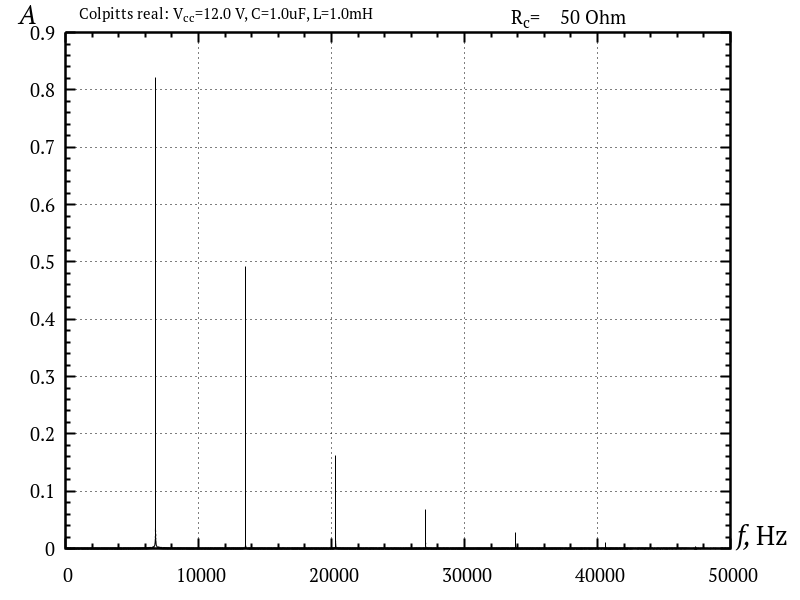
\includegraphics[width=0.48\textwidth]{p/r/f_050000.png}
  }
  \caption{Аттрактор и спектр реального генератора Колпитца при $R_c = \SI{50}{\ohm} $}
  \label{atu:f:colp_r_attr_f_50}
\end{figure}

При уменьшении значения $R_c$
происходит удвоение периода,
что отображается в виде второй петли аттрактора
и появлением приблизительно вдвое меньших частот в спектре~(рис.~\ref{atu:f:colp_r_attr_f_40}).

\begin{figure}[htb!]
  \centerline{
    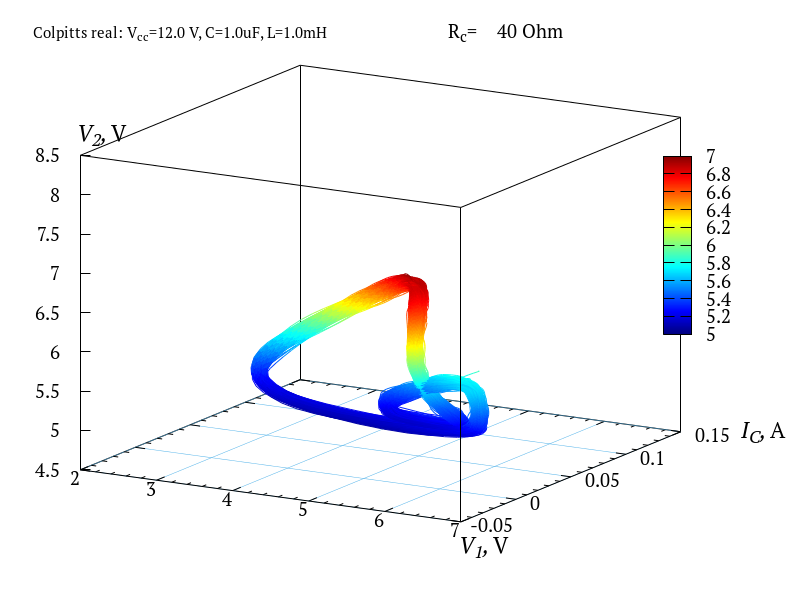
\includegraphics[width=0.48\textwidth]{p/r/v1iv2_040000.png}
    \hfill
    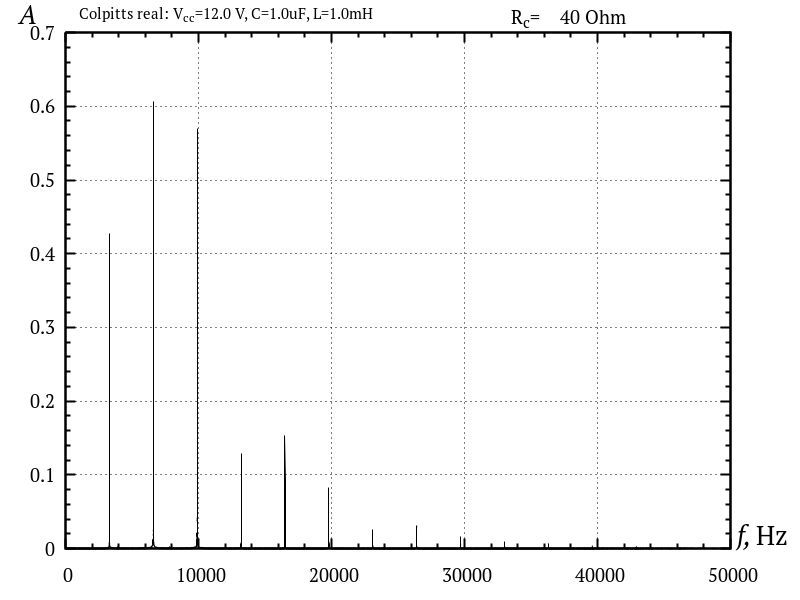
\includegraphics[width=0.48\textwidth]{p/r/f_040000.png}
  }
  \caption{Аттрактор и спектр реального генератора Колпитца при $R_c = \SI{40}{\ohm} $}
  \label{atu:f:colp_r_attr_f_40}
\end{figure}

Дальнейшее уменьшение значения параметра,
через каскад бифуркаций, приводит
к появлению странного аттрактора и сплошного спектра
(рис.~\ref{atu:f:colp_r_attr_f_30}).

\begin{figure}[htb!]
  \centerline{
    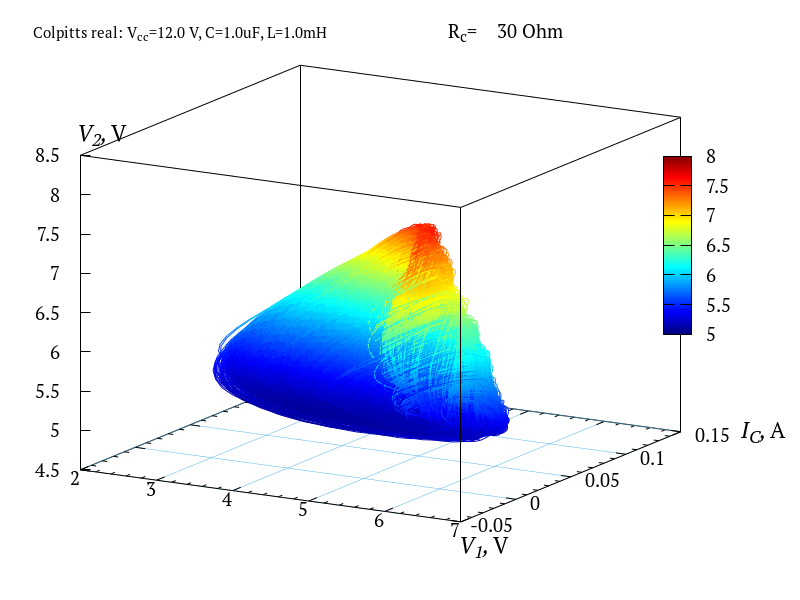
\includegraphics[width=0.48\textwidth]{p/r/v1iv2_030000.png}
    \hfill
    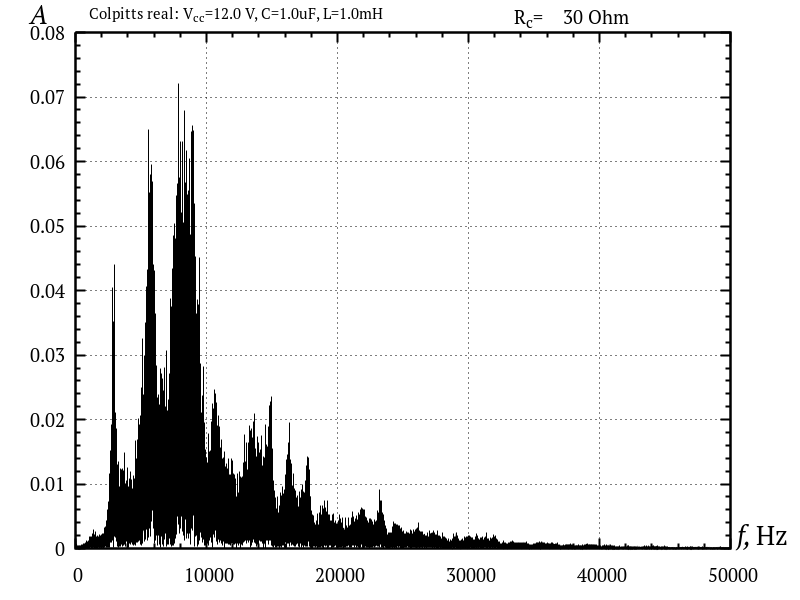
\includegraphics[width=0.48\textwidth]{p/r/f_030000.png}
  }
  \caption{Аттрактор и спектр реального генератора Колпитца при $R_c = \SI{30}{\ohm} $}
  \label{atu:f:colp_r_attr_f_30}
\end{figure}

При этом, в отличие от системы Лоренца,
при дальнейшем изменении параметра происходит чередование
хаотического и сложно-периодического режимов
(рис.~\ref{atu:f:colp_r_attr_f_29}).

\begin{figure}[htb!]
  \centerline{
    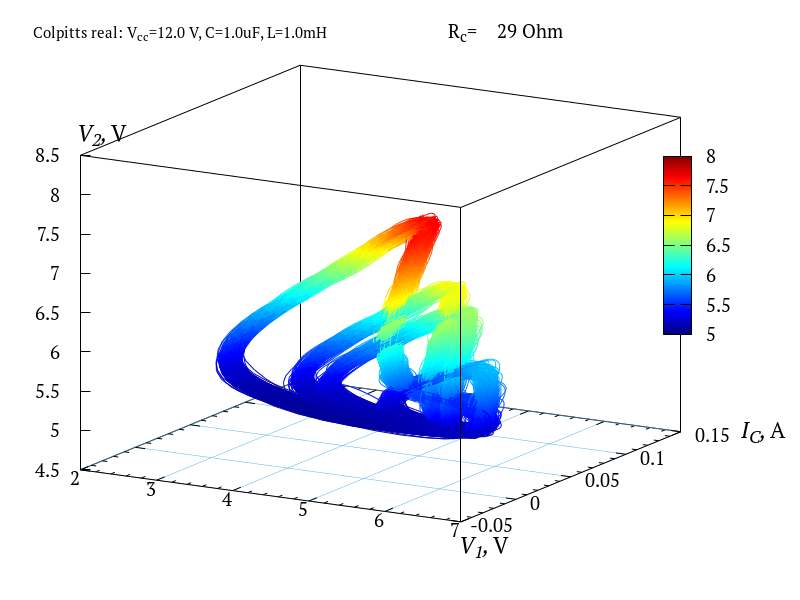
\includegraphics[width=0.48\textwidth]{p/r/v1iv2_029000.png}
    \hfill
    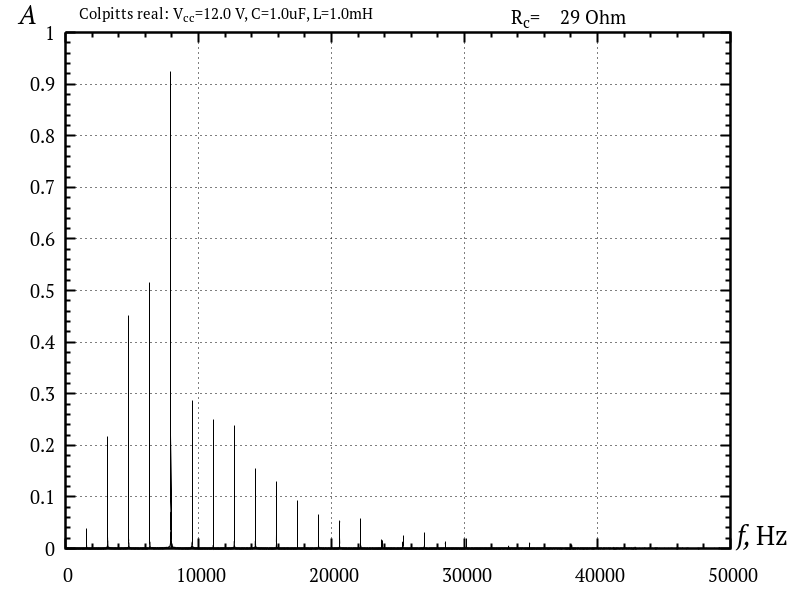
\includegraphics[width=0.48\textwidth]{p/r/f_029000.png}
  }
  \caption{Аттрактор и спектр реального генератора Колпитца при $R_c = \SI{29}{\ohm} $}
  \label{atu:f:colp_r_attr_f_29}
\end{figure}

В отличие от системы сбора данных, основанных на цифровом осциллографе,
разрешение в спектральной области составило $\SI{1}{\hertz}$,
что позволило уверенно отличать спектры хаотической
и сложно-периодической динамики.

% }}}1

\section{Анализ и выбор критериев}  % {{{1

При идентификации классической модели генератора Колпитца
был использован критерий $q_{x^2}$.
Замена модели на новую требует провести анализ критериев
повторно. На рис.~\ref{atu:f:colp_bjt_q-p_Rc_q}
представлены зависимости исследуемых критериев от значения $R_c$,
для новой модели.

\begin{figure}[htb!]
\centerline{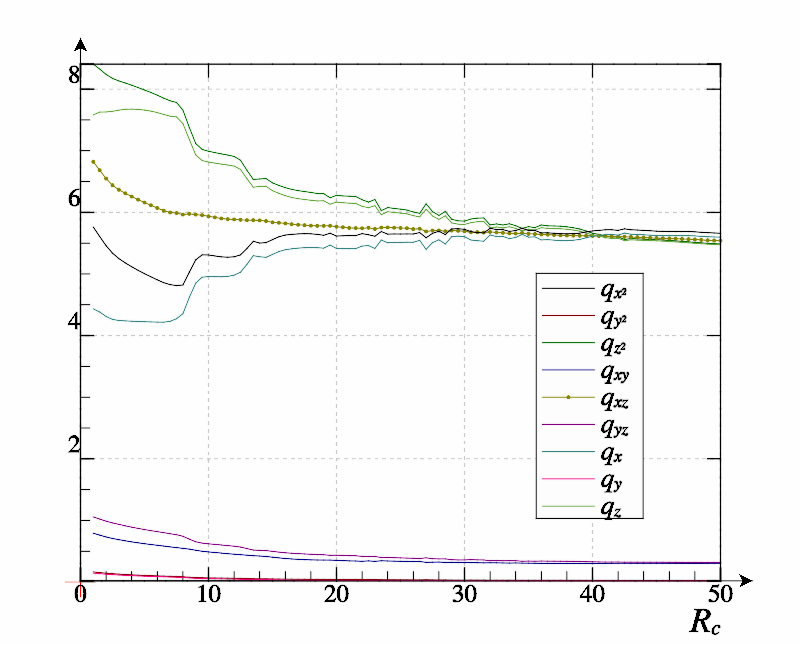
\includegraphics[width=0.7\textwidth]{p/colp_bjt_q-p_Rc_q.png} }
\caption{Зависимости значений критериев идентификации для модели системы Колпитца}
\label{atu:f:colp_bjt_q-p_Rc_q}
\end{figure}

Существенное нарушение монотонности как для ранее используемого
критерия $q_{x^2}$, так и для другого кандидата --- $q_{z^2}$,
особенно в областях, где наблюдается хаотическая динамика,
не способствует успешному процессу идентификации.
С другой стороны, критерий $q_{xz}$ проявляет
монотонную зависимость, по крайней мере для модели.

Рассмотрим зависимости этих же критериев, но для
реального генератора, полученные на основании данных
с предыдущей серии экспериментов с фиксированным значением
параметра. Полученные зависимости представлены на рис.~\ref{atu:f:colp_read_q-p_Rc_q-p_Rc_q}.


\begin{figure}[htb!]
\centerline{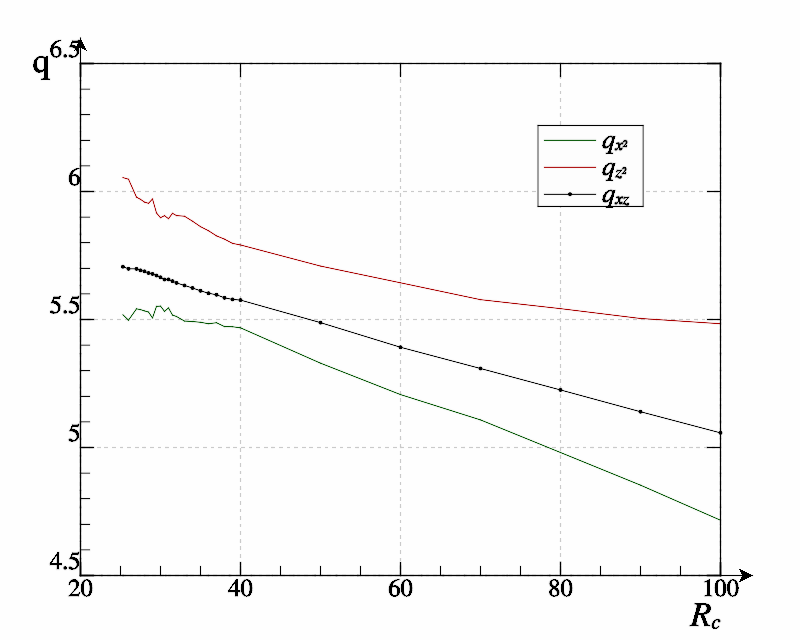
\includegraphics[width=0.7\textwidth]{p/colp_read_q-p_Rc_q.png} }
  \caption{Зависимости значений критериев идентификации $q_{x^2}$, $q_{z^2}$ и $q_{xz}$ для реального генератора Колпитца}
\label{atu:f:colp_read_q-p_Rc_q-p_Rc_q}
\end{figure}

Для реального генератора наблюдается картина, практически совпадающая
с результатами, полученными для модели. Таким образом,
критерий $q_{xz}$ потенциально является лучшим среди рассмотренных.

Для успешной идентификации необходима не только схожесть зависимостей критерия
от параметра для модели и объекта, но и близость их значений.
На рис.~\ref{atu:f:colp_q_cml} приведены зависимости $q_{xz}(R_c)$
как для объекта, так и для модели.

\begin{figure}[htb!]
\centerline{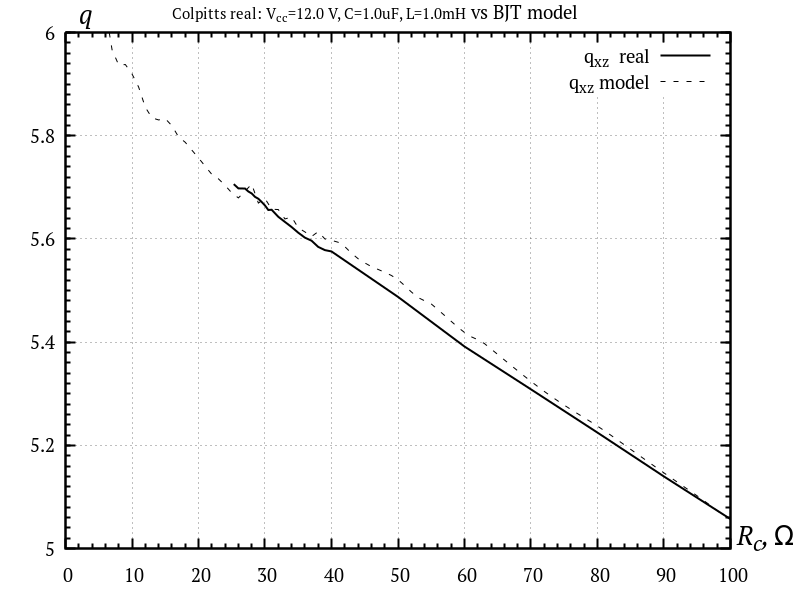
\includegraphics[width=0.7\textwidth]{p/colp_q_cml.png} }
\caption{Сравнение зависимостей значений критерия идентификации $q_{xz}$ реального генератора Колпитца с моделью}
\label{atu:f:colp_q_cml}
\end{figure}

Наблюдается хороший уровень совпадения, что свидетельствует не только
о правильности выбора критерия, но и о адекватности новой модели в  целом.
График зависимости для реального объекта имеет меньшую область определения,
что связано с физическими ограничениями конкретного объекта.

Несмотря на достаточную для работоспособности идентификации
близость графиков, следует отметить и определённые недостатки
данного критерия. Прежде всего, наблюдается практически одинаковое расстояние
между графиками при $R_c > \SI{40}{\ohm}$, то есть в тех областях,
где наблюдается регулярная динамика.
На основании имеющихся данных нет возможности определить,
чем конкретно вызвано это расхождение,
однако, следует предполагать заметную статическую ошибку идентификации
в этой области. Также, в пределах рабочей области значение критерия
изменяется слабо. Как следствие, ожидается повышенная чувствительность
идентификации к помехам при измерении.



% }}}1

\section{Синтез и анализ системы идентификации}  % {{{1

Для проверки работоспособности системы идентификации
в условиях нестационарного параметра, а также
для анализа характеристик этой системы,
необходимо обеспечить контролируемое изменение значения параметра.
Положение осложняется тем, что требуемые значения изменения сопротивления достаточно малы,
порядка единиц и десятков Ом, что исключает применение
цифровых потенциометров. Для реализации возможности изменять значение параметра
были предприняты следующие шаги.
К разъёму $\mathrm{P}_3$, была подключена дополнительна схема с независимым питанием,
состоящая из последовательно включенных переменного резистора
и MOSFET транзистора логического уровня и с малым сопротивлением
в открытом состоянии. Значение сопротивления переменного резистора
в каждом эксперименте подбиралось таки образом, чтобы
его сопротивление с учётом параллельного включения с резисторами $R_{cv1}$ и $R_{cv2}$
обеспечивало требуемое значение меньшого сопротивления,
а только $R_{cv1} + R_{cv2}$ --- большего.

Для управления включением MOSFET транзистора использовалось два подхода.
В первом транзистором управлял отдельный генератор на таймере 555.
Этот подход достаточно прост в реализации, однако
его применение усложняет задачу синхронизации при
определении ошибки идентификации. Поэтому
предпочтительным оказался второй подход,
при котором включением управлял сам контроллер через
оптическую развязку. Таким образом, переключения
происходили в заданные моменты времени,
привязанные к моменту запуска АЦП, что значительно упрощает
анализ ошибок идентификации. Общий вид установки для
проведения идентификации приведёт на рис.~\ref{atu:f:colp_r_id_dev}.
Часть элементов, например SDHC накопитель, находится под
другими частями установки, и не видна.


\begin{figure}[htb!]
  \centerline{
    \includegraphics[width=0.80\textwidth]{p/colp_stand.png}
  }
  \caption{Общий вид установки для идентификации нестационарного параметра $R_c$ реального генератора Колпитца }
  \label{atu:f:colp_r_id_dev}
\end{figure}

Естественным недостатком таких подходов является то, что
так можно обеспечить только скачкообразную динамику изменения параметра.
Однако, это не является принципиальным недостатком,
как как если система идентификации является работоспособной в таких условиях,
то она сохранит работоспособность и в случае плавного изменения параметра.

Для процессов параметрической идентификации генератора Колпитца представлены результаты четырёх экспериментов,
проведённых в схожих условиях.
Использовалась группа методов идентификации ``ql3rlWvnAAW''.

% C_1, C_2 = 1.0 uF, L = 1.0 mH, R_l=24.2 Ohm, R_e = 300 Ohm, R_1 = R_2 = 2.0 kOhm,
% Q: MMBT2222A: h_{FE}=210, V_{je} = 0.667V.
% V_{cc} = 12.0 V, V_{b} = 5.94 V
% d_0.txt: 27.0 - 50.0 Ohm  28.5  +-  11.5
% d_1.txt: 29.5 - 35.0 Ohm  32.25 +-  2.75
% d_2.txt: 32.0 - 40.0 Ohm  36.0  +-  4.0
% d_3.txt: 28.0 - 37.0 Ohm  32.5  +-  4.5
% old:
% d_0.txt: 27.3 - 44.2 Ohm  35.75 +-  8.45
% d_1.txt: 29.0 - 35.0 Ohm  32    +-  3
% d_2.txt: 26.0 - 30.0 Ohm  28    +-  2
% d_3.txt: 31.0 - 52.0 Ohm  41.5  +- 10.5
% d_4.txt: 29.0 - 32.0 Ohm  30.5  +-  1.5

Параметры первого эксперимента для генератора Колпитца
%
\begin{equation}
  \begin{array}{c}
    R_{c,\min} = \SI{27.0}{\ohm};
    \;
    R_{c,\max} = \SI{50.0}{\ohm};
    \;
    T_{R_c} = \SI{200}{\milli\second};
  \\
    R_c(t) = \SI{28.5}{\ohm} + \SI{11.5}{\ohm} \cdot \sign \sin \left(  \frac{\pi t}{T_{R_c}}  \right)
  \end{array}
  \label{atu:eq:colp_test1_cond}
\end{equation}
%
были подобраны таки образом, что бы изменение значения параметра
приводило к переходу от хаотического режима к периодическому.

Как видно из графиков, отображающих процесс идентификации~(рис.~\ref{atu:f:colp_r_id_1}),
система идентификации оказалась вполне работоспособной.


\begin{figure}[htb!]
  \centerline{
    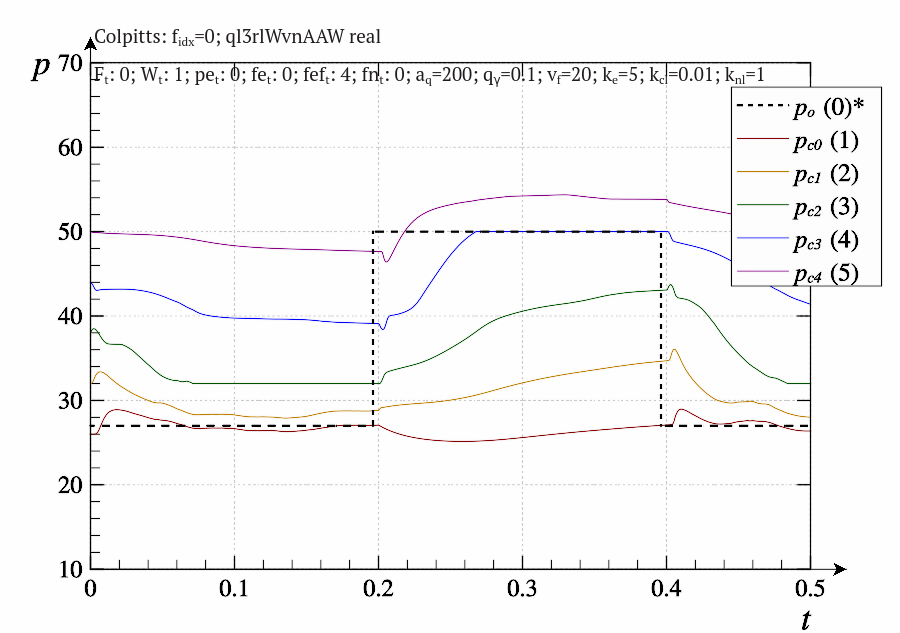
\includegraphics[width=0.48\textwidth]{p/r/colp_real_id-p_t_pi_ql3rlWvnAAW_real_d_0.png}
    \hfill
    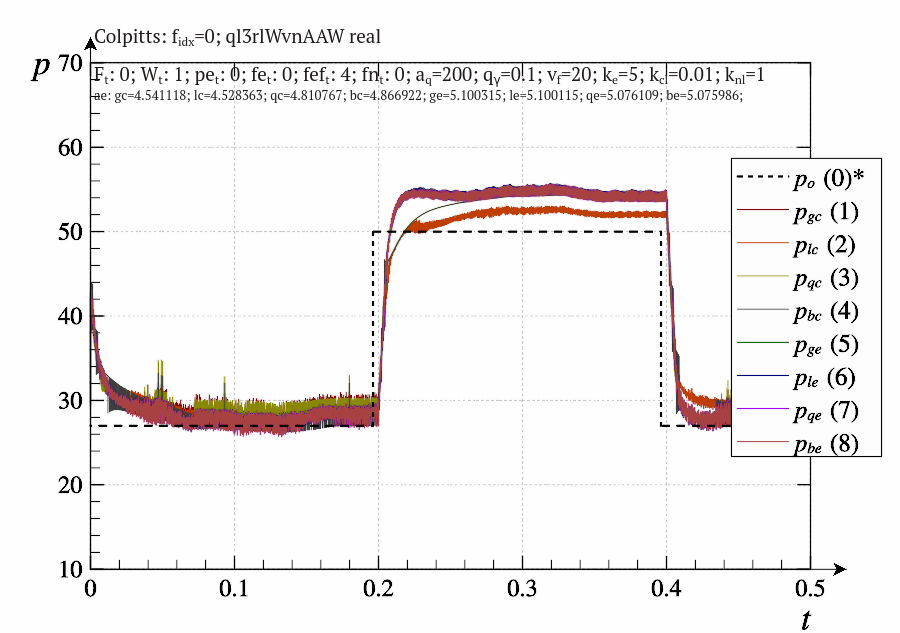
\includegraphics[width=0.48\textwidth]{p/r/colp_real_id-p_t_p_ql3rlWvnAAW_real_d_0.png}
  }
  \caption{Процесс идентификации параметра $R_c$ реального генератора Колпитца при условиях (\ref{atu:eq:colp_test1_cond})}
  \label{atu:f:colp_r_id_1}
\end{figure}

При этом следует отметить значительную ошибку идентификации при $R_c = \SI{50}{\ohm}$.
Её появление следовало ожидать, с учётом уже упомянутой разницы
в значениях критерия для объекта и модели.
При этом наблюдается достаточно редкое явление --- одну из
наименьших ошибок идентификации показал метод координатора поиска
$p_{gc}$. Это связано с тем, что этот метод характеризуется
смещением идентифицируемого значения к центру рабочей области
в случаях, когда идентифицируемое значение находится вблизи края
этой области. Таким образом, одна ошибка скомпенсировала другую.
Однако, это достаточно редкий частный случай, и не стоит
рассматривать полученный результат как преимущество метода $p_{gc}$.


Параметры второго эксперимента для генератора Колпитца
%
\begin{equation}
  \begin{array}{c}
    R_{c,\min} = \SI{29.5}{\ohm};
    \;
    R_{c,\max} = \SI{35.0}{\ohm};
    \;
    T_{R_c} = \SI{200}{\milli\second};
  \\
    R_c(t) = \SI{32.25}{\ohm} + \SI{2.75}{\ohm} \cdot \sign \sin \left( \frac{\pi t}{T_{R_c}}  \right)
  \end{array}
  \label{atu:eq:colp_test2_cond}
\end{equation}
%
соответствуют переключена динамики системы меду хаотическим
и сложно периодическим режимами.

Результаты моделирования процессов идентификации,
представленные на рис.~\ref{atu:f:colp_r_id_2},
отображают не только сохранение работоспособности,
но и уменьшение ошибки идентификации из-за работы на том участке критерия,
на котором различие между объектом и моделью минимально.


\begin{figure}[htb!]
  \centerline{
    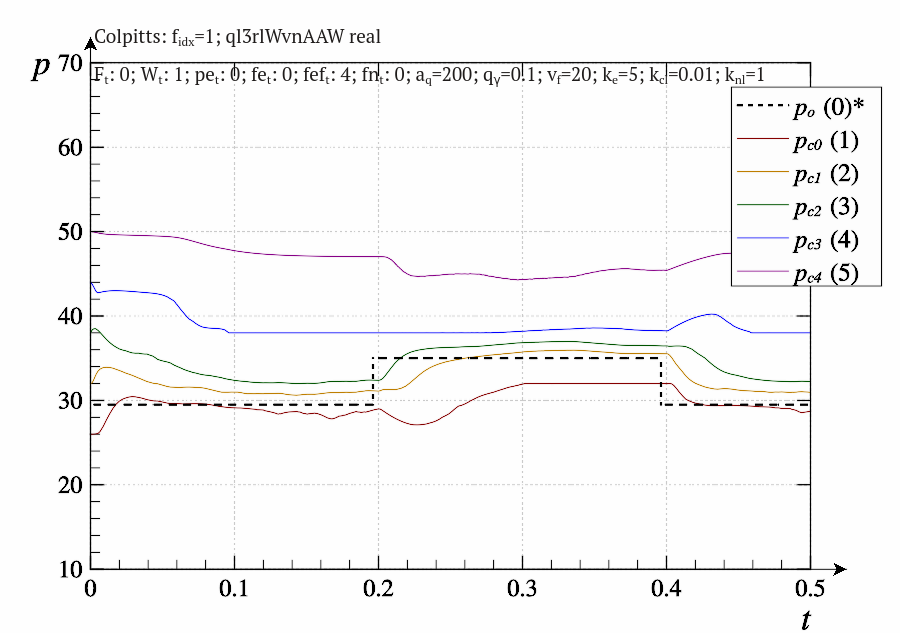
\includegraphics[width=0.48\textwidth]{p/r/colp_real_id-p_t_pi_ql3rlWvnAAW_real_d_1.png}
    \hfill
    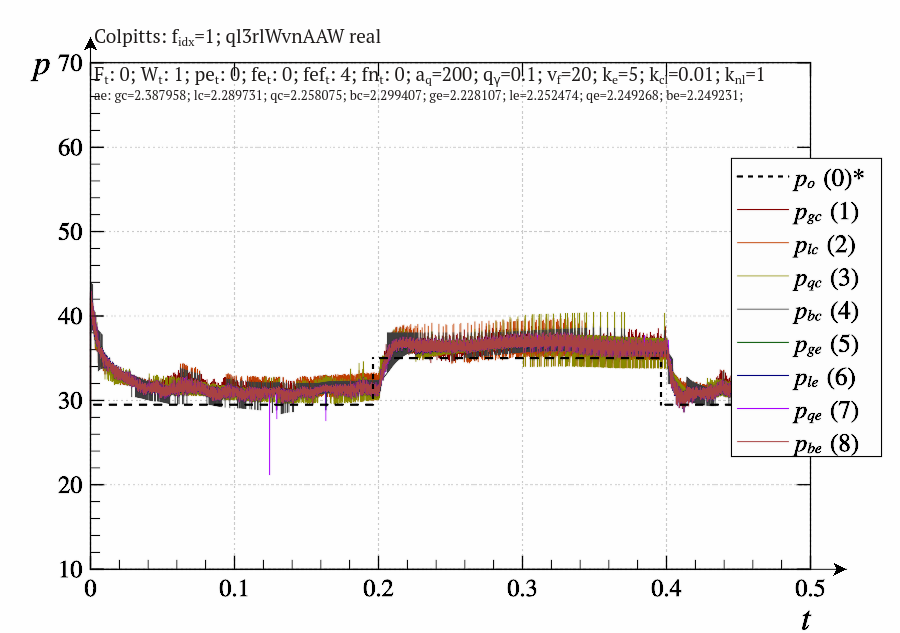
\includegraphics[width=0.48\textwidth]{p/r/colp_real_id-p_t_p_ql3rlWvnAAW_real_d_1.png}
  }
  \caption{Процесс идентификации параметра $R_c$ реального генератора Колпитца при условиях (\ref{atu:eq:colp_test2_cond})}
  \label{atu:f:colp_r_id_2}
\end{figure}


Параметры третьего эксперимента для генератора Колпитца
%
\begin{equation}
  \begin{array}{c}
    R_{c,\min} = \SI{32.0}{\ohm};
    \;
    R_{c,\max} = \SI{40.0}{\ohm};
    \;
    T_{R_c} = \SI{200}{\milli\second};
  \\
    R_c(t) = \SI{36.0}{\ohm} + \SI{4.0}{\ohm} \cdot \sign \sin \left(   \frac{\pi t}{T_{R_c}}   \right)
  \end{array}
  \label{atu:eq:colp_test3_cond}
\end{equation}
%
соответствуют переходу между двумя сложно-периодическими режимами
с различным колоченом петлей в аттракторе.

При этом процесс идентификации (рис.~\ref{atu:f:colp_r_id_3}) оказался подвержен
той же ошибке, которая наблюдалась в первом эксперименте,
хотя в целом процесс идентификации протекает нормально.


\begin{figure}[htb!]
  \centerline{
    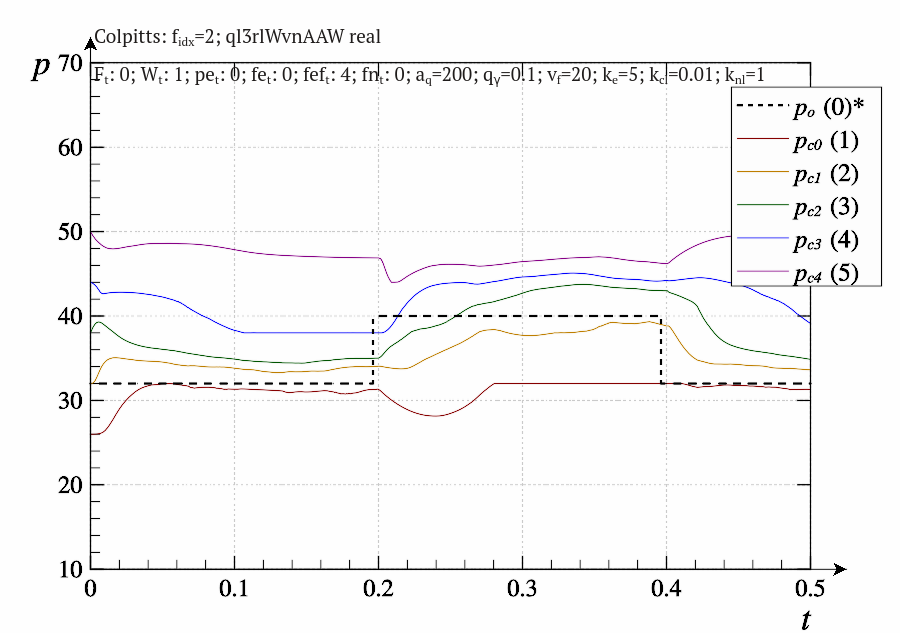
\includegraphics[width=0.48\textwidth]{p/r/colp_real_id-p_t_pi_ql3rlWvnAAW_real_d_2.png}
    \hfill
    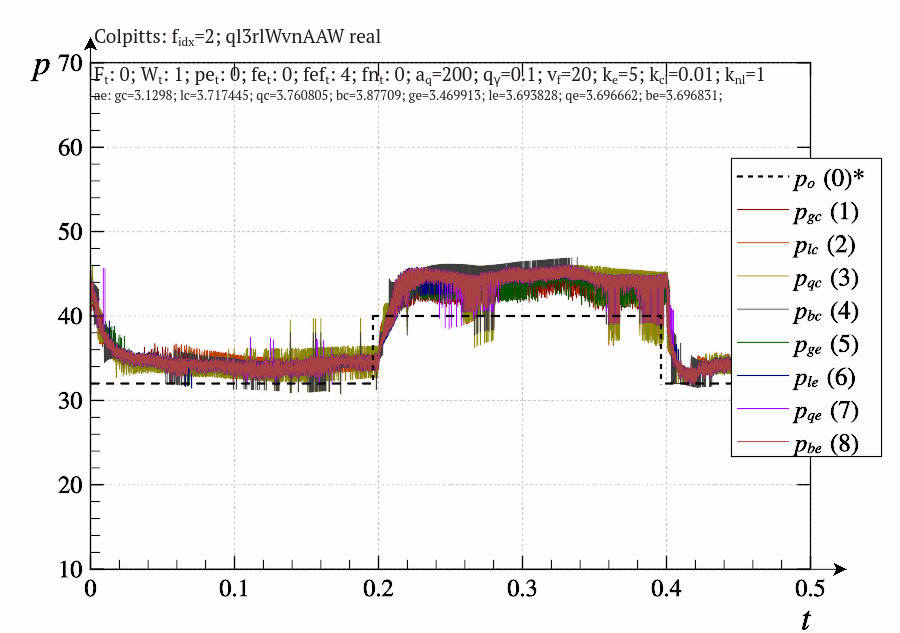
\includegraphics[width=0.48\textwidth]{p/r/colp_real_id-p_t_p_ql3rlWvnAAW_real_d_2.png}
  }
  \caption{Процесс идентификации параметра $R_c$ реального генератора Колпитца при условиях (\ref{atu:eq:colp_test3_cond})}
  \label{atu:f:colp_r_id_3}
\end{figure}



Параметры четвёртого эксперимента для генератора Колпитца
%
\begin{equation}
  \begin{array}{c}
    R_{c,\min} = \SI{28.0}{\ohm};
    \;
    R_{c,\max} = \SI{37.0}{\ohm};
    \;
    T_{R_c} = \SI{200}{\milli\second};
  \\
    R_c(t) = \SI{32.5}{\ohm} + \SI{4.5}{\ohm} \cdot \sign \sin \left( \frac{\pi t}{T_{R_c}}  \right).
  \end{array}
  \label{atu:eq:colp_test4_cond}
\end{equation}
%
в какой-то мере аналогичны параметрам из второго эксперимента.
Происходит переключение из хаотического режима в сложно-периодический,
но амплитуда изменения параметра несколько больше.

Так как в данном эксперименте
(рис.~\ref{atu:f:colp_r_id_4})
не происходит попадание в область,
где зависимости критерия для модели и объекта заметно отличаются,
то и ошибка идентификации меньше, чем в первом и третьем эксперименте.

\begin{figure}[htb!]
  \centerline{
    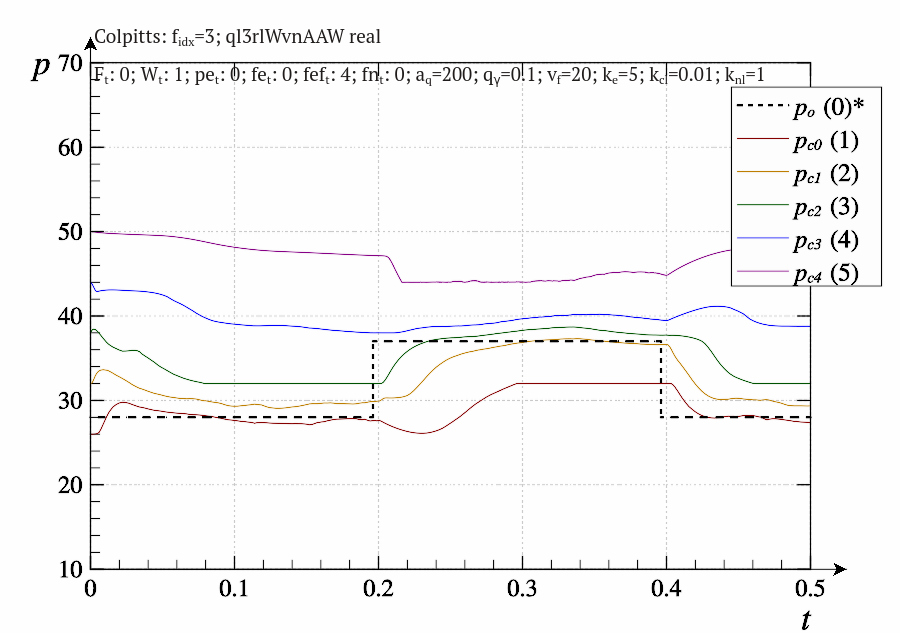
\includegraphics[width=0.48\textwidth]{p/r/colp_real_id-p_t_pi_ql3rlWvnAAW_real_d_3.png}
    \hfill
    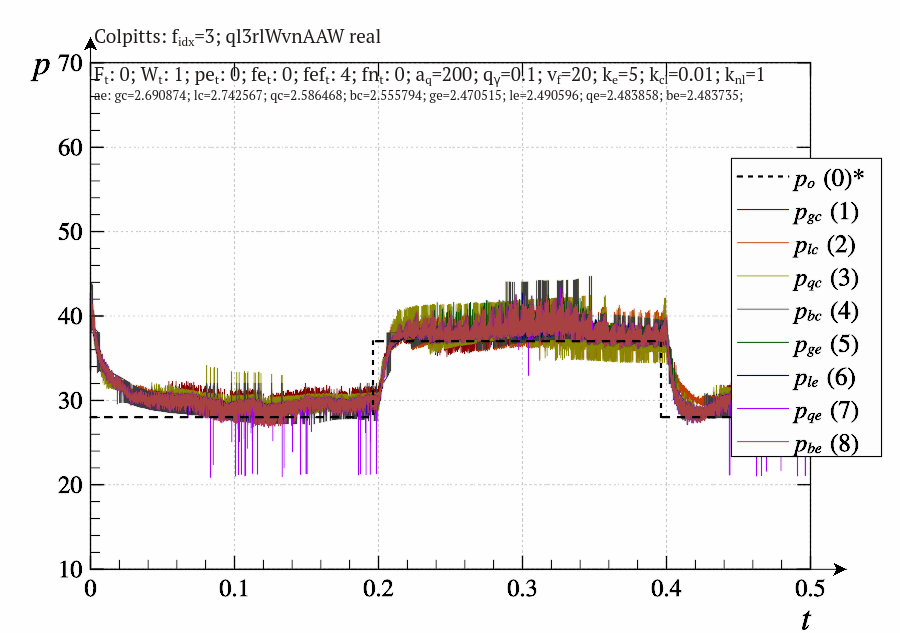
\includegraphics[width=0.48\textwidth]{p/r/colp_real_id-p_t_p_ql3rlWvnAAW_real_d_3.png}
  }
  \caption{Процесс идентификации параметра $R_c$ реального генератора Колпитца при условиях (\ref{atu:eq:colp_test4_cond})}
  \label{atu:f:colp_r_id_4}
\end{figure}

Таким образом, для всех четырёх экспериментов система идентификации
с использованием группы методов ``ql3rlWvnAAW'' и критерия $q_{xz}$
показала свою работоспособность. Ошибки идентификации при этом
в первую очередь обусловлены существующей разницей в динамике
объекта и моделей, а не недостатками метода.


% }}}1

\section{Влияние параметров системы идентификации на ошибку идентификации для реального генератора Колпитца}  % {{{1


Рассмотрим зависимости ошибок идентификации от параметров самой системы идентификации.
Параметр $a_q$, задающий
фильтрующие способности критерия идентификации, должен рассматриваться в первую очередь.
На рис.~\ref{atu:f:colp_real_id_p_a_q_d_0} представлены полученные зависимости
для процессов идентификации параметра $R_c$ генератора Колпитца.

\begin{figure}[htb!]
  \centerline{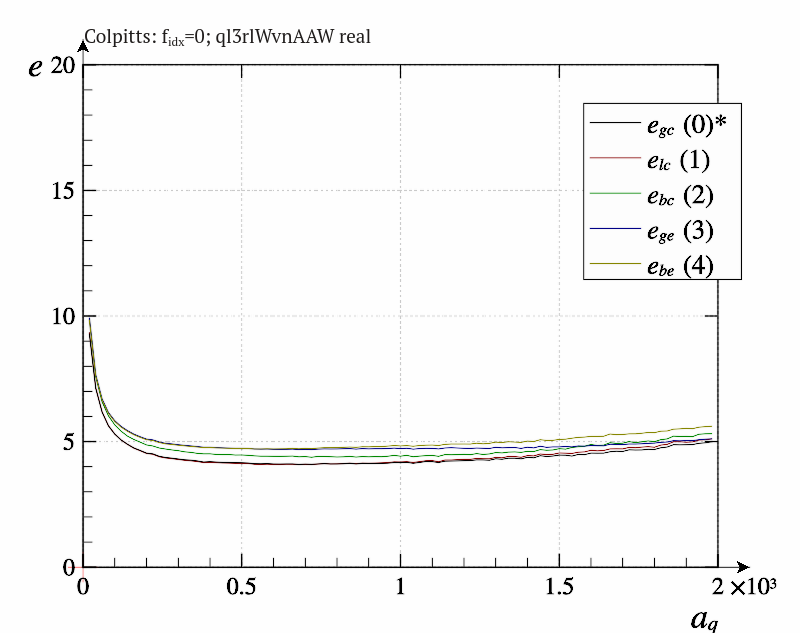
\includegraphics[width=0.6\textwidth]{p/r/colp_real_id-p_a_q_d_0.png} }
  \caption{Зависимости $\overline{e}(a_q)$ при идентификации параметра $R_c$ генератора Колпитца при условиях \ref{atu:eq:colp_test1_cond} }
  \label{atu:f:colp_real_id_p_a_q_d_0}
\end{figure}


\begin{figure}[htb!]
  \centerline{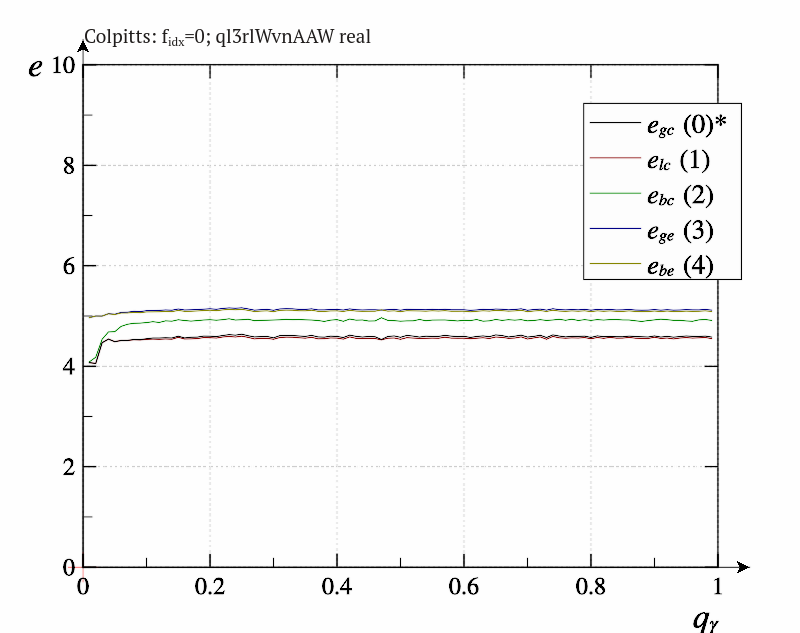
\includegraphics[width=0.6\textwidth]{p/r/colp_real_id-p_q_gamma_d_0.png} }
  \caption{Зависимости $\overline{e}(q_\gamma)$ при идентификации параметра $R_c$ генератора Колпитца при условиях \ref{atu:eq:colp_test1_cond} }
  \label{atu:f:colp_real_id_p_q_gamma_d_0}
\end{figure}

\begin{figure}[htb!]
  \centerline{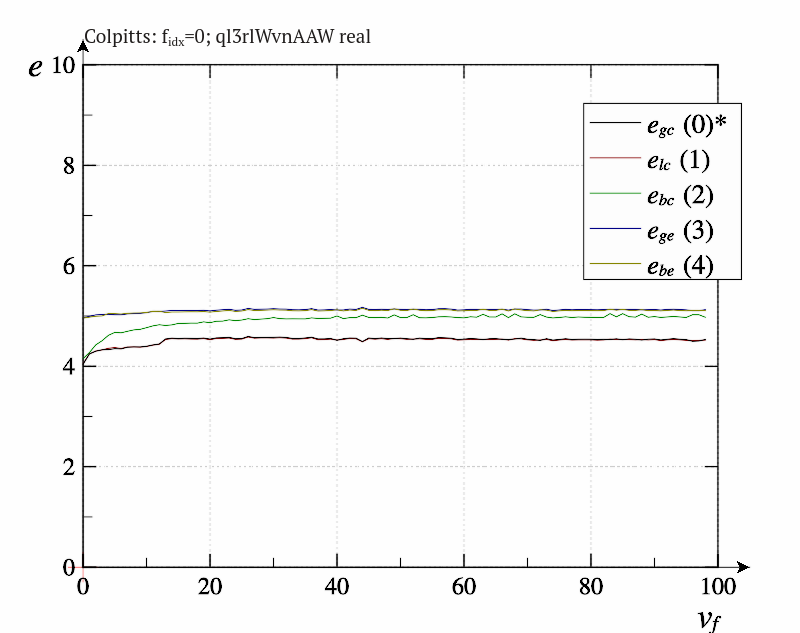
\includegraphics[width=0.6\textwidth]{p/r/colp_real_id-p_v_f_d_0.png} }
  \caption{Зависимости $\overline{e}(v_f)$ при идентификации параметра $R_c$ генератора Колпитца при условиях \ref{atu:eq:colp_test1_cond} }
  \label{atu:f:colp_real_id_p_v_f_d_0.png}
\end{figure}


\begin{figure}[htb!]
  \centerline{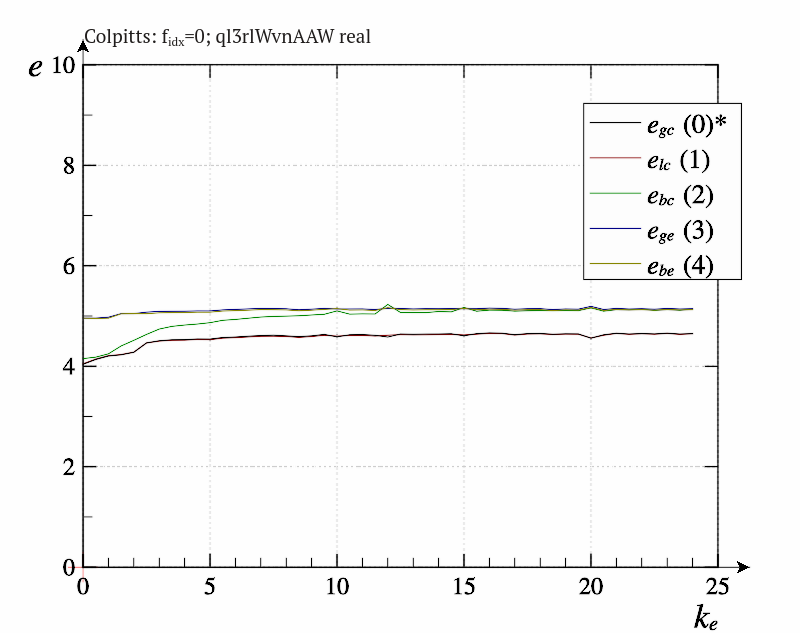
\includegraphics[width=0.6\textwidth]{p/r/colp_real_id-p_k_e_d_0.png} }
  \caption{Зависимости $\overline{e}(k_e)$ при идентификации параметра $R_c$ генератора Колпитца при условиях \ref{atu:eq:colp_test1_cond} }
  \label{atu:f:colp_real_id_p_k_e_d_0.png}
\end{figure}


\begin{figure}[htb!]
  \centerline{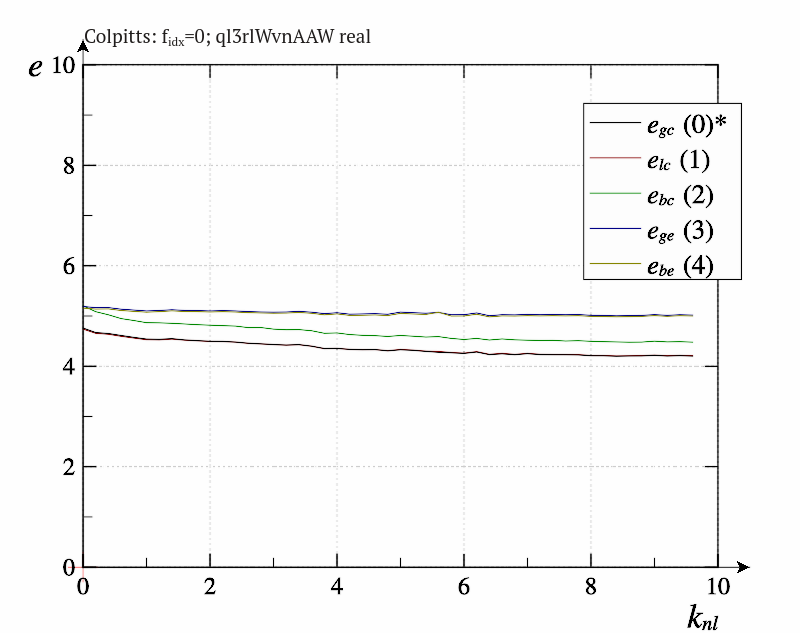
\includegraphics[width=0.6\textwidth]{p/r/colp_real_id-p_k_nl_d_0.png} }
  \caption{Зависимости $\overline{e}(k_{nl})$ при идентификации параметра $R_c$ генератора Колпитца \ref{atu:eq:colp_test1_cond} }
  \label{atu:f:colp_real_id_p_k_nl_d_0.png}
\end{figure}
%
%
% \begin{figure}[htb!]
%   \centerline{\includegraphics[width=0.6\textwidth]{p/colp_real_id_qi_fv5_prm_0-p_k_cn.png} }
%   \caption{Зависимости $\overline{e}_{r*}(c_n)$ при идентификации параметра $R_c$ генератора Колпитца}
%   \label{atu:f:colp_real_id_qi_fv5_prm_0-p_k_cn.png}
% \end{figure}

% }}}1


\section{Выводы по разделу \thechapter}  % {{{1


В целом синтез критерия идентификации и построение работоспособной системы идентификации для
системы генератора Колпитца не потребовало никаких специальных подходов и введения дополнительных
мер оценивания взаимосвязей параметров генератора.

% }}}1

% vim: fdm=marker foldlevel=0 foldignore="%#" fdc=4 ft=tex
